%==============================================================================
% USGLoc -- Extended Report (companion to the RA-L letter usgloc_ral_draft.tex).
%
% Purpose: report EVERYTHING that does not fit the 6-page letter -- full
% implementation detail, the evidential-head (EDL) training analysis with
% measured numbers, map statistics, the retrieval-training study, extended
% result tables (per-scene calibration, full ablations, robustness, runtime),
% and the SGLoc-protocol comparison the letter cites as supplementary.
% This file doubles as the arXiv extended version / reviewer supplementary.
% Build: pdflatex -> bibtex -> pdflatex -> pdflatex (same toolchain as the letter).
%==============================================================================
\documentclass[journal]{IEEEtran}

\usepackage{amsmath,amssymb,amsfonts,bm}
\usepackage{graphicx}
\graphicspath{{figures/}}
\usepackage{xcolor}
\usepackage{booktabs}
\usepackage{cite}
\usepackage{url}
\usepackage{tikz}
\usetikzlibrary{positioning,arrows.meta,backgrounds,fit,calc}
\usepackage{orcidlink}
\usepackage[subpreambles=false]{standalone}

% ---- Shared colors for the \input'ed TikZ figures ----
\definecolor{ink}{HTML}{273746}
\definecolor{uLow}{HTML}{1B9E77}
\definecolor{uMid}{HTML}{E6AB02}
\definecolor{uHigh}{HTML}{D95F02}
\definecolor{coarseBg}{HTML}{EAF2FB}
\definecolor{coarseLn}{HTML}{9DC3EC}
\definecolor{fineBg}{HTML}{FDF1E6}
\definecolor{fineLn}{HTML}{F0C28E}
\definecolor{encBg}{HTML}{EEF6EE}
\definecolor{encLn}{HTML}{B7D8B7}
\definecolor{outBg}{HTML}{FFF3D6}
\definecolor{outLn}{HTML}{D9A300}
\definecolor{poseC}{HTML}{2E6FAC}
\definecolor{mapprin}{HTML}{E8F4EF}
\definecolor{mappt}{HTML}{F2F3F4}
\definecolor{locpt}{HTML}{EAF2FB}
\definecolor{ourstr}{HTML}{FFF3D6}

\newcommand{\res}{{\color{red}\textbf{--}}}
\newcommand{\TODO}[1]{{\color{red}[TODO: #1]}}
\newcommand{\figbox}[2]{%
  \fbox{\parbox[c][#1][c]{0.93\linewidth}{\centering\footnotesize #2}}}
\newcommand{\method}{USGLoc}

\begin{document}

\title{Supplementary Material for \\ \method{}: Uncertainty-Aware Semantic
Visual Localization from 3D Gaussian Splatting}

\author{Thanh Nguyen Canh\orcidlink{0000-0001-6332-1002},~\IEEEmembership{Graduate Student Member,~IEEE},
Bang Nguyen Van, Xiem HoangVan, and Nak Young Chong\orcidlink{0000-0001-5736-0769},~\IEEEmembership{Senior Member,~IEEE}
\thanks{This work was supported by JST SPRING, Japan Grant Number JPMJSP2102.
(Corresponding authors: nakyoung@jaist.ac.jp, xiemhoang@vnu.edu.vn)}
\thanks{Thanh Nguyen Canh and Nak Young Chong are with the Japan Advanced
Institute of Science and Technology, Ishikawa 923-1211, Japan.}
\thanks{Bang Nguyen Van and Xiem HoangVan are with the University of
Engineering and Technology, Vietnam National University, Hanoi 10000, Vietnam.}}

\markboth{Extended report accompanying the RA-L submission}%
{Nguyen Canh \MakeLowercase{\textit{et al.}}: \method{} Extended Report}

\maketitle

%------------------------------------------------------------------------------
\begin{abstract}
This extended report accompanies the \method{} letter. The letter presents an
evidential localization framework on a 3D Gaussian Splatting (3DGS) map,
built on one principle: the map's own uncertainty should drive every stage of
localization and survive to the output. This report documents everything the
letter's page budget excludes. We give the complete implementation and
training recipes, an empirical analysis of the shared evidential head (EDL),
statistics of the evidential map, a study of retrieval-encoder training on
real data, per-scene calibration breakdowns, the full ablation grid, the
robustness sweeps, per-stage runtime, and the DSLAM-protocol comparison with
SGLoc referenced by the letter. Eight implementation findings are reported; three of them we believe transfer to other evidential-perception systems:
(i) an EDL head's classification accuracy converges long before its
uncertainty structure does; (ii) a shared head must be trained on its full
deployment distribution --- both input domains AND all scenes --- or the
unseen part's evidence collapses; and (iii) viewpoint submaps must be
frustum-culled, or retrieval descriptors of a room-scale scene collapse onto
a single vector.
\end{abstract}

\begin{IEEEkeywords}
Localization, semantic scene understanding, uncertainty quantification,
evidential deep learning, Gaussian splatting.
\end{IEEEkeywords}

%------------------------------------------------------------------------------
\section{Scope and Relation to the Letter}
The RA-L letter (\emph{\method{}: Uncertainty-Aware Semantic Visual
Localization from 3D Gaussian Splatting}) is the primary publication: it
motivates the problem, derives the method (evidential map, vacuity-gated
matching, vacuity-weighted refinement, tempered Laplace posterior), and
reports the headline benchmark results. This report is the companion record.
Section~\ref{sec:impl} fixes every implementation detail. Sections
\ref{sec:edl}--\ref{sec:retrieval} analyze the three learned components with
measured numbers. Sections \ref{sec:protocol}--\ref{sec:sgloc} hold the
extended evaluation. Nothing here repeats the letter: the method, the pipeline
overview and the headline tables are in the letter and are not reproduced.
Where a table extends one of the letter's, the caption says so.

%------------------------------------------------------------------------------
\section{Implementation Details}
\label{sec:impl}

\subsection{Offline map training}
Each scene is trained by a four-stage pipeline (\texttt{scripts/train\_map.py}
in the released code); Table~\ref{tab:mapcfg} lists every hyperparameter.
Gaussians are initialized by back-projecting the depth maps of every 25th
mapping frame at a stride of 8 pixels, voxel-deduplicated at 2\,cm, and capped
at 200k seeds. The photometric fit uses gsplat rasterization~\cite{kerbl3dgs} with
DefaultStrategy densification, plain RGB colors (no spherical harmonics), and
an L1 loss at $320{\times}240$ for 7{,}000 iterations, one random view per
iteration over every 10th mapping frame. Semantic distillation runs FastSAM~\cite{fastsam}
masks with CLIP~\cite{clip} ViT-B/16 crop embeddings on every 20th frame; each mask's
embedding is accumulated onto the Gaussians whose centres project inside the
mask, pass a depth-occlusion test ($|z-d|<0.15$\,m), and lie in front of the
camera. On chess this yields 329{,}028 Gaussians, of which 94\% receive at
least one semantic observation from 9{,}348 mask embeddings; the full
pipeline takes \textbf{94\,s} on an RTX~5070~Ti (16\,GB) at
$320{\times}240$, and 140--370\,s at $640{\times}480$.

\begin{table}[t]
\caption{Map-training configuration (identical for all scenes).}
\label{tab:mapcfg}
\centering\scriptsize
\setlength{\tabcolsep}{3pt}
\begin{tabular}{@{}lll@{}}
\toprule
Stage & Parameter & Value \\
\midrule
Init & frame / pixel stride & 25 / 8 \\
     & voxel dedup / cap & 2\,cm / 200k \\
Fit  & iterations @ resolution & 7{,}000 @ $320{\times}240$ \\
     & \quad or (4 scenes, Sec.~\ref{sec:mapres}) & 20{,}000 @ $640{\times}480$ \\
     & frame stride / loss & 10 (5 at $640{\times}480$) / L1 \\
     & densify start--stop / reset & 500--4{,}000 / 3{,}000 \\
     & lr (means$^{*}$, quats, scales) & $1.6{\times}10^{-4*}$, $10^{-3}$, $5{\times}10^{-3}$ \\
     & lr (opacities, colors) & $5{\times}10^{-2}$, $2.5{\times}10^{-3}$ \\
Distill & frame stride / occlusion tol. & 20 / 0.15\,m \\
        & CLIP / segmenter & ViT-B/16 laion2b / FastSAM-s \\
Opinions & full-evidence count $n_0$ & 4 \\
Instances & voxel $\times$ class & 0.4\,m $\times$ argmax class \\
\bottomrule
\multicolumn{3}{@{}l@{}}{\footnotesize $^{*}$scaled by the scene extent, as in 3DGS.}
\end{tabular}
\end{table}

\subsection{Open-vocabulary class set}
The evidential class count is $C{=}25$:
\emph{wall, floor, ceiling, door, window, chair, sofa, table, desk, shelf,
cabinet, monitor, keyboard, mouse, book, cup, bottle, plant, lamp, stairs,
curtain, box, bag, kitchen appliance, sink}. Class prototypes are CLIP text
embeddings of ``\emph{a photo of a $\langle$class$\rangle$ in a room}''.
Pseudo-labels are the argmax cosine similarity, kept only when the
top-1/top-2 margin exceeds 0.01.

%------------------------------------------------------------------------------
\section{The Shared Evidential Head}
\label{sec:edl}

The head is a two-layer MLP ($512 \to 256 \to C$, softplus output,
$\sim$138k parameters, 550\,KB on disk) mapping CLIP features to Dirichlet
evidence. It is trained once, then frozen and shared by the map and query
sides. Neither FastSAM nor CLIP is fine-tuned.

\subsection{Training data and schedule}
\label{sec:edl-training}
The head needs \emph{no manually labeled dataset}: its training set is
generated automatically from the mapping frames themselves during map
building, and Table~\ref{tab:edl-setup} lists the full configuration. Two
feature domains are pooled across ALL scenes (the reasons are Finding~2,
Sec.~\ref{sec:edl-domains}). \emph{Mask domain}: every FastSAM mask crop
embedded by CLIP on the distillation frames of every scene --- 17{,}175
confidence-filtered embeddings over the seven 7Scenes environments (per
scene 504--5{,}375). \emph{Gaussian domain}: the per-Gaussian mask-averaged
features of the already-mapped scenes, subsampled to at most 20k observed
Gaussians per scene --- 23{,}556 after filtering (chess + fire) ---
40{,}731 training features in total. The trained head reaches 70--86\%
pseudo-label agreement on every scene's mask bank with the vacuity ordering
intact. Labels are CLIP zero-shot pseudo-labels: cosine
similarity against the $C{=}25$ text prototypes (``\emph{a photo of a
$\langle$class$\rangle$ in a room}''), argmax kept only when the
top-1/top-2 margin exceeds 0.01; ambiguous features are deliberately
excluded so the head assigns them little evidence at inference, which is
the desired vacuity behavior. Optimization uses the EDL loss~\cite{edl}
(letter, Eq.~7): the Dirichlet Brier risk plus a KL regularizer toward the
uniform Dirichlet on the misleading evidence, annealed as
$\lambda_t = \min(1, \mathrm{epoch}/10)$. Training takes seconds; the head is then frozen for the benchmark's
scenes and both sides of the pipeline (a new benchmark, e.g. 12Scenes,
gets its own pooled head from its own mapping frames). When a scene
is mapped with a frozen head, stage~4 skips training entirely and only
applies the head.

\begin{table}[t]
\caption{EDL head: complete training configuration (chess numbers).}
\label{tab:edl-setup}
\centering\scriptsize
\setlength{\tabcolsep}{3pt}
\begin{tabular}{@{}ll@{}}
\toprule
Item & Value \\
\midrule
architecture & MLP $512{\to}256{\to}25$, ReLU, softplus \\
parameters / size & $\sim$138k / 550\,KB \\
training set & 40{,}731 CLIP features (auto-generated) \\
\quad mask domain & 17{,}175 crops, ALL 7 scenes \\
\quad Gaussian domain & 23{,}556 sampled (mapped scenes) \\
labels & CLIP zero-shot vs.\ 25 prototypes, argmax \\
label filter & top-1/top-2 cosine margin $> 0.01$ \\
loss & EDL: Brier risk + annealed KL~\cite{edl} \\
KL anneal & $\lambda_t = \min(1, \mathrm{epoch}/10)$ \\
optimizer / lr / batch & Adam / $10^{-3}$ / 512 \\
epochs & 40 (Sec.~\ref{sec:edl-epochs}: why not 10) \\
wall-clock & seconds (RTX 5070 Ti) \\
reuse & trained once per benchmark, frozen; shared \\
\bottomrule
\end{tabular}
\end{table}

\subsection{Finding 1: uncertainty structure needs more epochs than accuracy}
\label{sec:edl-epochs}
On a controlled toy problem (4 orthonormal class directions in
$\mathbb{R}^{16}$, 5\% feature noise), classification accuracy exceeds 90\%
within ${\sim}10$ epochs, but the property the vacuity gate relies on ---
\emph{ambiguous inputs earn more vacuity than clean ones} --- is absent at 20
epochs and only emerges by 60 (Table~\ref{tab:edl-epochs}). We therefore
train for 40 epochs by default and regression-test the ordering.

\begin{table}[t]
\caption{Mean vacuity $u$ and top-class belief vs.\ training epochs.
``Mix'' = 50/50 mixtures of two class prototypes (the ambiguous regime);
``junk'' = random unit vectors.}
\label{tab:edl-epochs}
\centering\footnotesize
\setlength{\tabcolsep}{3.5pt}
\begin{tabular}{@{}lcccccc@{}}
\toprule
& \multicolumn{3}{c}{20 epochs} & \multicolumn{3}{c}{60 epochs} \\
\cmidrule(lr){2-4}\cmidrule(lr){5-7}
& clean & mix & junk & clean & mix & junk \\
\midrule
vacuity $u$ & 0.631 & 0.632 & 0.629 & 0.677 & \textbf{0.710} & 0.703 \\
top belief $b_{\max}$ & 0.119 & 0.107 & 0.104 & \textbf{0.223} & 0.136 & 0.111 \\
\bottomrule
\end{tabular}
\end{table}

\subsection{Finding 2: the shared head must train on both input domains}
\label{sec:edl-domains}
The head is applied to raw mask-crop CLIP features (query side) and to
per-Gaussian features averaged over many overlapping masks (map side).
Averaging shifts features off the raw-mask manifold. A head trained only on
mask features assigns the averages near-zero evidence: on chess the median
per-Gaussian vacuity was 0.997 \emph{despite 94\% observation coverage}, and
the primitive-level spread collapsed (Table~\ref{tab:dual-domain}) --- the
gate had nothing to discriminate. Training the same head on the union of both
domains (each pseudo-labeled identically) restores a full spread at no
architectural cost.

The same lesson holds \emph{across scenes}: a dual-domain head trained on
chess alone reached only 8.9\% pseudo-label agreement on fire's features,
and fire's map evidence collapsed exactly as above (median vacuity 0.994).
Pooling the training set over all scenes (Sec.~\ref{sec:edl-training})
restores 70--86\% agreement everywhere. We regard this as a general caution
for shared evidential heads: \emph{share the weights, and share the full
training distribution --- every input domain and every environment the head
will score}.

\begin{table}[t]
\caption{Chess map vacuity with a mask-only vs.\ dual-domain head.
$u_{\mathrm{eff}}$ is the fused primitive-level effective vacuity
(letter, Sec.~III-A); $q_p$ denotes quantiles.}
\label{tab:dual-domain}
\centering\footnotesize
\setlength{\tabcolsep}{3.5pt}
\begin{tabular}{@{}lcc@{}}
\toprule
 & mask-only head & dual-domain head \\
\midrule
per-Gaussian median $u$ & 0.997 & 0.761 \\
per-Gaussian $q_{10}$ & 0.995 & 0.223 \\
primitive $u_{\mathrm{eff}}$ $q_{10}/q_{25}/q_{50}$ & 0.82 / 0.89 / 0.99 & 0.001 / 0.26 / 0.97 \\
primitives with $u_{\mathrm{eff}}{<}0.7$ & 8 / 1916 & 629 / 1916 \\
primitives with $u_{\mathrm{eff}}{<}0.1$ & 0 / 1916 & 402 / 1916 \\
\bottomrule
\end{tabular}
\end{table}

\subsection{Evidence scaling and fusion behavior}
Per-Gaussian evidence is scaled by observation count,
$e \leftarrow e \cdot \min(1, n/n_0)$ with $n_0{=}4$: a never-observed
Gaussian has $u{=}1$ exactly, and evidence accumulates with support, as
subjective logic prescribes. Note that with $C{=}25$ classes the
\emph{per-observation} vacuity floor is high ($u = C/S$), which is not a
defect: cluster-level DST fusion multiplies member vacuities, so agreement
across members compounds into confidence (the bimodal primitive distribution
of Table~\ref{tab:dual-domain}), while disagreement routes conflict into
vacuity under Yager's rule~\cite{yager,dst}. The absolute scale is absorbed by the gate
sharpness $\lambda_u$ and pixel-weight sharpness $\gamma$; only the ordering
matters, which Sec.~\ref{sec:edl-epochs} verifies.

%------------------------------------------------------------------------------
\section{Evidential Map Statistics}
\label{sec:mapstats}
Table~\ref{tab:mapstats} summarizes the per-scene maps. Each map trains in
60--95\,s on an RTX 5070 Ti. The per-\emph{Gaussian} median vacuity is high
by construction: with $C{=}25$ classes an unobserved or singly-observed
Gaussian is near-fully vacuous, and most Gaussians are seen from few
distillation frames. What the localizer consumes is the per-\emph{primitive}
effective vacuity after cluster-level Yager fusion, which recovers a
confident low-vacuity population from the observed minority: every scene has
hundreds of object primitives with $u_\text{eff}<0.5$ for the gate and the
pixel weight to act on.

\begin{table}[t]
\caption{Per-scene evidential map statistics (SfM pseudo-GT poses).
``obs.'' is the fraction of Gaussians receiving $\ge 1$ semantic
observation; ``masks'' the FastSAM/CLIP embeddings distilled; ``$u_\text{eff}
{<}0.5$'' the count of low-vacuity object primitives the gate uses.}
\label{tab:mapstats}
\centering\scriptsize
\setlength{\tabcolsep}{3pt}
\begin{tabular}{@{}lccccc@{}}
\toprule
Scene & splats & prims & obs. & masks & prims $u_\text{eff}{<}0.5$ \\
\midrule
chess      & 329k & 2{,}384 & 94\% & 9{,}348  & 696 \\
fire       & 188k & 1{,}113 & 96\% & 2{,}891  & 455 \\
heads      & 246k & 607     & 84\% & 1{,}218  & 103 \\
office     & 437k & 3{,}174 & 89\% & 10{,}637 & 574 \\
pumpkin    & 252k & 2{,}164 & 97\% & 6{,}585  & 280 \\
redkitchen & 387k & 3{,}351 & 92\% & 14{,}464 & 542 \\
stairs     & 289k & 1{,}770 & 96\% & 1{,}320  & 659 \\
\bottomrule
\end{tabular}
\end{table}

\subsection{Finding 3: render fidelity gates registration, and fitting
resolution must be chosen per scene}
\label{sec:mapres}
The map is not only a geometric model, it is the \emph{image source} the
matcher registers against, so its render fidelity bounds the whole system.
We quantify this with two per-map measurements on train-side frames
(Table~\ref{tab:maprestab}): the render PSNR at the ground-truth pose, and
the \emph{correction floor}, the error the matching correction attains when
started from the true pose --- the best the localizer could ever do on that
map.

Refitting at the matcher's own resolution ($640{\times}480$, 20k iterations,
every 5th frame, versus $320{\times}240$/7k/every 10th) is \emph{not}
uniformly better. On the four smaller scenes it raises PSNR and lowers the
floor, on Chess from 0.569 to 0.379\,cm. On Heads, Office and Redkitchen it does the opposite: Redkitchen loses 3.5\,dB, Office 2.5\,dB and Heads 1.9\,dB, because the
higher-resolution objective produces roughly twice as many Gaussians whose
geometry is less well converged, and sharp-but-misplaced detail registers
worse than a smooth approximation. Raising the iteration budget does not
recover it; refitting Redkitchen at 60k iterations instead of 20k left PSNR unchanged to within 0.1\,dB, so this is not an optimization-budget effect.

The operational consequence is the sharper result. Registration rate --- the
fraction of frames on which the correction succeeds at all --- tracks render
PSNR with a threshold near 20\,dB: every selected map above it registers on 90--100\% of frames (the two unselected fits above 20\,dB, Heads at $640{\times}480$ and the Office intermediate fit, register on 85\% and 80\%), while Redkitchen's high-resolution variant at 18.1\,dB registers on
only 65\%, and Office's at 19.6\,dB on 75\%. A map can therefore have a
\emph{better} floor and still be the worse choice: Redkitchen at high
resolution more than halves the floor (1.071 to 0.463\,cm) yet fails to
register on a third of frames, which the pipeline can only answer with the
photometric fallback. We therefore select the fitting resolution per scene on
train-side frames, ranking by registration rate and breaking ties by floor;
the test split plays no part in the choice. Four scenes select the
high-resolution fit and three the original one.

\begin{table}[t]
\caption{Map fitting resolution, chosen per scene on TRAIN-side frames (20
per scene). ``PSNR@GT'' is the render fidelity at the ground-truth pose,
``floor'' the correction error from a ground-truth initialization, and
``reg.'' the fraction of frames the correction registers at all. The
selected variant is bold.}
\label{tab:maprestab}
\centering\scriptsize
\setlength{\tabcolsep}{3.5pt}
\begin{tabular}{@{}lcccccc@{}}
\toprule
& \multicolumn{3}{c}{$320{\times}240$ fit} & \multicolumn{3}{c}{$640{\times}480$ fit} \\
\cmidrule(lr){2-4}\cmidrule(lr){5-7}
Scene & PSNR & floor & reg. & PSNR & floor & reg. \\
\midrule
chess      & 22.98 & 0.569 & 100\% & \textbf{23.87} & \textbf{0.379} & \textbf{100\%} \\
fire       & 24.64 & 0.712 & 100\% & \textbf{25.51} & \textbf{0.471} & \textbf{100\%} \\
pumpkin    & 26.33 & 1.427 & 100\% & \textbf{26.87} & \textbf{1.103} & \textbf{100\%} \\
stairs     & 26.71 & 1.771 & 100\% & \textbf{27.77} & \textbf{1.413} & \textbf{100\%} \\
\midrule
heads      & \textbf{24.73} & \textbf{0.328} & \textbf{100\%} & 22.87 & 0.406 & 85\% \\
office     & \textbf{22.08} & \textbf{1.874} & \textbf{90\%}  & 19.61 & 1.203 & 75\% \\
redkitchen & \textbf{21.62} & \textbf{1.071} & \textbf{100\%} & 18.14 & 0.463 & 65\% \\
\bottomrule
\end{tabular}
\end{table}

We validated the ranking criterion end to end rather than trusting the
proxies. Office is the scene where floor and registration rate disagree most
sharply, so we also built an intermediate fit ($480{\times}360$, 15k
iterations): it improves the correction floor and keeps render fidelity above the 20\,dB threshold (20.8\,dB), yet it registers on
80\% of frames against 90\% for the selected map. End to end it is substantially worse, 3.35 against 1.59\,cm, because the fifth of queries it
cannot register fall back to the photometric path. Registration rate is
therefore the correct primary criterion and the floor only a tie-break: a
map must first be one the matcher can use at all.

A practical corollary for any render-and-match localizer: report the render
fidelity of the map, not only the pose error. The floor and the registration
rate together explain the per-scene accuracy spread far better than any
parameter of the pose estimator, both are measurable without ever touching
the test split, and of the two it is the registration rate that must be
optimized first.

%------------------------------------------------------------------------------
\section{Retrieval-Encoder Training on Real Data}
\label{sec:retrieval}

The retrieval front end went through three redesigns, each forced by a
measured failure on the held-out test split. We report them because each is a
concrete, transferable lesson. Together with the matching correction of
Sec.~\ref{sec:correction-full}, they moved the chess test median from
61.5\,cm to 0.69\,cm (Table~\ref{tab:retrieval-ladder}).

\begin{table}[t]
\caption{Retrieval-front-end fix ladder (chess, test split). Each row adds one change to the row above. Rows 1--4 are historical 40-query measurements on the earlier $320{\times}240$ map; rows 5--7 are 100-query runs.}
\label{tab:retrieval-ladder}
\centering\footnotesize
\setlength{\tabcolsep}{4pt}
\begin{tabular}{@{}lcc@{}}
\toprule
Configuration & med.\ (cm) & SR@5/5 \\
\midrule
$\pm$offset InfoNCE variants, single-scale refine & 61.50 & 2\% \\
\;+ Voronoi-assigned positives & 47.00 & 5\% \\
\;+ hierarchical CLIP shortlist + evidential rerank & 13.40 & 40\% \\
\;+ coarse-to-fine pyramid + triage & 6.20 & 45\% \\
\;+ evidential matching correction (Sec.~\ref{sec:correction-full}) & 0.69 & 97\% \\
\;+ per-scene map resolution (Sec.~\ref{sec:mapres}) & 0.55 & 86\% \\
\;+ fidelity-verified snaps, inlier weights, mode (Table~I) & \textbf{0.56} & \textbf{88\%} \\
\bottomrule
\end{tabular}
\end{table}

\subsection{Finding 4: submaps must be frustum-culled}
With radius-only submaps ($r{=}3$\,m) in a room smaller than the radius,
every chess submap contained 768--1{,}529 of the 2{,}384 primitives; all
reference scene descriptors collapsed onto one vector (pairwise cosine
0.9996--1.0000) and the symmetric InfoNCE loss sat exactly at chance,
$\ln(24) \approx 3.178$, for 400 iterations. Culling each submap to the
primitives that project into its anchor view (in front of the camera, inside
the image) yields 154--340 primitives per submap with Jaccard overlap
${\sim}0.40$ between neighboring anchors. This mirrors the covisibility
submaps of SGLoc~\cite{sgloc}: viewpoint content, not a distance ball, is the
retrieval unit.

\subsection{Finding 5: positives must be uniquely assigned}
Our first contrastive design drew positives from frames within a pose radius
of each anchor. Because neighboring anchors overlap, one frame was a positive
for several anchors at once, so the in-batch InfoNCE saw the same frame as
both positive and negative and collapsed to chance ($\ln 24$). Assigning
every mapping frame to exactly one nearest anchor (a pose-space Voronoi
partition, with a small view-angle penalty) removes the contradiction: the
loss converges to 0.82, and this is the change that first moved test accuracy
off the floor. Fixed $\pm$offset variants (near-identical views 0.1\,s apart)
also failed to generalize --- validation median 1.9\,cm but test 61\,cm ---
because they carry none of the cross-sequence viewpoint change the test split
has; frames drawn from an anchor's whole Voronoi cell supply it.

\subsection{Finding 6: retrieval must be viewpoint-robust, refinement
coarse-to-fine}
Two geometric facts about 7Scenes drove the final design. First, held-out
test sequences run ${\sim}13$--$15$\,cm off the mapping trajectory
\emph{regardless} of anchor spacing (the nearest anchor to a chess test frame
is 13.5\,cm away even at a 5-frame stride), so any anchor-based initialization
starts the refiner more than 10\,cm from the answer. Second, single-scale
$320{\times}240$ refinement has a convergence basin of only ${\sim}10$\,cm; a
$80{\times}60 \to 160{\times}120 \to 320{\times}240$ pyramid widens it to
20--35\,cm (measured from perturbed ground truth). We therefore (i) replace
the instance-only submap ranking with a CLIP whole-image shortlist reranked
by the evidential gated similarity --- the gate keeps its role, the global
descriptor adds viewpoint robustness at no training cost --- and (ii) triage
the top-8 shortlisted hypotheses through the cheap first pyramid stage,
continuing the best $K{=}3$ by render fidelity. The remaining gap to
sub-centimeter methods was a feature-matching pose correction (as in
GS-CPR~\cite{gscpr}). Section~\ref{sec:correction-full} adds exactly that
stage, driven by the same evidential channel, and closes the gap.

%------------------------------------------------------------------------------
\section{The Evidential Matching Correction}
\label{sec:correction-full}

\subsection{Why a correction stage: bimodal failure, detectable but
unrecoverable}
The pyramid architecture of Sec.~\ref{sec:retrieval} produced a
characteristic error distribution on the test split: photometric refinement
either converges to sub-centimeter accuracy or fails completely, with almost
nothing in between. On chess (seed 0, 100 queries) the 10th-percentile error
was 0.5\,cm and 34\% of queries landed under 2\,cm, yet 29\% ended beyond
20\,cm; fire showed the same shape with a larger success mode. The reported medians (7.54 and 2.66\,cm) sat in the valley between the two modes. Two
further measurements defined the fix. First, the failures are
\emph{detectable}: final render fidelity separates converged from failed
queries at 96--97\% accuracy (threshold ${\approx}18$\,dB PSNR), so the
pipeline knows when it failed but had no mechanism to recover. Second, the
failures are \emph{initialization} failures: they cluster in contiguous
test-sequence segments whose viewpoints sit outside the photometric
convergence basin of every retrieved anchor.

\subsection{Mechanism and measured basin}
The correction stage (letter, Sec.~III-D) renders the map at the hypothesis
pose (RGB, expected depth, and vacuity in one rasterization pass), matches
the query against the render with frozen LoFTR~\cite{loftr} indoor weights,
gates the correspondences by the rendered vacuity, lifts the surviving
render-side keypoints to 3D through the rendered depth, and solves PnP-RANSAC with LM refinement, iterated for five rounds.
Table~\ref{tab:corr-basin} shows the measured basin on three chess test
frames: the correction recovers 30\,cm/15$^\circ$ initializations on every
frame and 60\,cm/25$^\circ$ on most, an order of magnitude beyond the
photometric pyramid, at ${\sim}0.25$\,s per hypothesis. From a perfect
initialization it converges to 0.3--0.6\,cm, which is the geometric noise
floor of the rendered map itself and sets the accuracy ceiling of the full
system. Failure is clean: when no matches survive the gate, the pose is
returned unchanged and the hypothesis falls back to the photometric path.

On the full benchmark (100 queries per scene, median of 3 seeds) the effect
is decisive. Chess drops from 7.54 to \textbf{0.55}\,cm (0.22$^\circ$), Fire from 2.66 to \textbf{0.57}\,cm, Heads from 4.74 to \textbf{0.56}\,cm, and the seven-scene average from 14.9 to \textbf{2.51}\,cm in translation and from 3.9 to \textbf{0.36}$^\circ$ in rotation (the pre-correction numbers are seed 0). These are the numbers after the per-scene map selection of Sec.~\ref{sec:mapres} but before the fidelity check on corrected poses and the inlier-based weights, which bring the average to 1.25\,cm, and before the fine-tune and agreement weight of Sec.~\ref{sec:final}, which bring it to 1.05\,cm (Table~\ref{tab:ace}). The correction snaps 94--100\% of queries on every scene, 73--80\% of Chess, Fire and Heads queries land under 1\,cm, and median localization time falls from ${\sim}29$\,s to 5.3--7.0\,s because snapped hypotheses skip the pyramid.

\begin{table}[t]
\caption{Measured correction basin (chess test frames; pose perturbed from
ground truth by the stated magnitude, then corrected). Entries are final
translation errors in cm; ``---'' = correction reported failure (pose
unchanged, photometric fallback).}
\label{tab:corr-basin}
\centering\footnotesize
\setlength{\tabcolsep}{4pt}
\begin{tabular}{@{}lccccc@{}}
\toprule
init offset & 0 & 10\,cm/5$^\circ$ & 30\,cm/15$^\circ$ & 60\,cm/25$^\circ$ & 100\,cm/40$^\circ$ \\
\midrule
seq-03/121 & 0.60 & 0.94 & 1.31 & 1.92 & --- \\
seq-05/030 & 0.59 & 1.44 & 1.21 & ---  & --- \\
seq-03/500 & 0.33 & 1.53 & 2.06 & 3.63 & --- \\
\bottomrule
\end{tabular}
\end{table}

\subsection{Finding 7: snap rate, not snap accuracy, sets per-scene error}
\label{sec:snaprate}
Per-scene results separate cleanly by one statistic: the fraction of
queries the correction successfully snaps (Table~\ref{tab:snaprate}).
Scenes that snap every query reach 0.5--0.9\,cm, and the three scenes with
unsnapped queries are the three least accurate, because an unsnapped
hypothesis reverts to the photometric pyramid and inherits its failure mode. Stairs is the extreme case, and it is instructive. Its correction
\emph{floor} --- the error obtained by correcting from ground truth itself
--- is 1.41\,cm on the selected map (Table~\ref{tab:snaprate}; 1.77\,cm on the $320{\times}240$ map), comparable to office, so neither the matcher nor the map geometry prevents a good answer. What fails is the frequency of snapping:
repetitive tread geometry yields few confident, mutually consistent
matches (median 72 inliers, versus 1{,}156 on chess).

Two interventions were measured. Refitting the map at the matcher's
resolution ($640{\times}480$, 20k iterations, every 5th frame) improved the correction floor on stairs from 1.77 to 1.41\,cm (Table~\ref{tab:maprestab}) but, measured before the fidelity check, moved the snap rate only from 37\% to 40\%: map fidelity bounds how \emph{well} a snap lands,
not how \emph{often} one happens. Loosening the match gates raised the snap
rate substantially (50\% to 78\% on perturbed stairs frames) but degraded
the error tail, because PnP on a repeated structure can be confident and
wrong --- large inlier counts on the wrong tread. We therefore keep the
loosened gates and add an independent fidelity check: a corrected pose
takes a mixture slot only when it renders better than the anchor it started
from, and snapped candidates are ranked by render fidelity rather than by
inlier count. Rejected candidates return to the photometric path rather
than being discarded, so the mixture never loses a component. On Stairs
this raises the snap rate from 69\% to 96\% and lowers the median error
from 12.89 to 8.25\,cm, with rotation from 2.10$^\circ$ to 1.17$^\circ$ and
coverage from 27/33/42 to 36/50/55; on Office the snap rate rises from
78\% to 92\% and the median falls from 2.37 to 2.22\,cm. Neither costs
runtime (\texttt{results/verify\_seed0}). The general
lesson is that \emph{inlier count is not a trust signal on repetitive
geometry}; an independent appearance check is required, and in a
rendering-based localizer it is already available for free.

Stairs remains the hardest scene even so: its \emph{snapped} queries carried a 6.1\,cm median error before the fidelity check and still carry 2.8\,cm in the reported run. The correction is not failing randomly but
landing on the wrong tread of a self-similar staircase, which renders
almost as well as the right one. This is the irreducible part of the
problem for a retrieval-initialized render-and-match localizer, and it is
precisely the regime the pose mixture exists to express: the scene admits
several poses of comparable evidence, and the honest output is a
distribution over them rather than a confident point.

\begin{table}[t]
\caption{Snap rate versus accuracy (seed 0, 100 queries). ``floor'' is the
correction error from ground-truth initialization, i.e.\ the map's geometric limit, measured on the 20 mapping-side frames of Table~\ref{tab:maprestab} (test-frame floors are in Table~\ref{tab:headroom}); ``inl'' the median gated inlier count.}
\label{tab:snaprate}
\centering\footnotesize
\setlength{\tabcolsep}{4pt}
\begin{tabular}{@{}lccccc@{}}
\toprule
Scene & snap & med.\ (cm) & $\le$1\,cm & floor (cm) & inl \\
\midrule
chess      & 100\% & 0.47 & 79\% & 0.39 & 2{,}363 \\
fire       & 100\% & 0.51 & 80\% & 0.37 & 2{,}950 \\
heads      & 100\% & 0.56 & 73\% & 0.36 & 1{,}612 \\
redkitchen & 100\% & 0.85 & 58\% & 0.66 & 1{,}897 \\
office     & 99\% & 1.35 & 28\% & 1.01 & 1{,}067 \\
stairs     & 99\% & 2.39 & 16\% & 1.24 & 550 \\
pumpkin    & 98\% & 1.15 & 45\% & 0.95 & 1{,}460 \\
\bottomrule
\end{tabular}
\end{table}

\subsection{Configuration}
LoFTR (\texttt{indoor\_new}, ScanNet-trained) runs at $640{\times}480$, its
native training resolution and the native 7Scenes format. The confidence
threshold is written into the matcher's own configuration rather than
applied afterwards: kornia's LoFTR filters at its internal coarse threshold
before returning anything, so a smaller value applied downstream would never
act. Matches require
matcher coarse confidence $\ge 0.2$, render alpha $\ge 0.5$, rendered depth $\ge 0.1$\,m,
a local $3{\times}3$ depth spread $\le 10\%$ of the depth (expected depth
blends surfaces at silhouettes, so matches near a discontinuity lift
phantom 3D points), and \emph{alpha-normalized} rendered vacuity
$U_r/\alpha_r \le u_{\max}{=}0.9$ (the evidential gate; ablated by
\texttt{--no-corr-gate}). The normalization matters: the blended vacuity
channel is bounded by the render alpha, so an unnormalized threshold of
0.9 would only ever fire at near-opaque pixels and the gate would be
structurally inert. Keypoints follow the rasterizer's pixel-center
convention (index $+\,0.5$) on both sides of PnP, and depth is sampled
bilinearly at the subpixel keypoint. PnP-RANSAC uses a 2\,px reprojection
threshold, 2{,}000 iterations, and confidence 0.9999, followed by
Levenberg--Marquardt refinement on the inliers. A correction round is
accepted with $\ge 8$ inliers, and across rounds the solution with the
most inliers is kept (a later round can regress on a degenerate re-render).
Snapped hypotheses are deduplicated by camera-centre distance (1\,cm) and
rotation angle ($2^\circ$), with the duplicate's retrieval mass merged into
the kept hypothesis, then re-ranked by render fidelity
(Sec.~\ref{sec:snaprate}). Each receives a
shortened final photometric refinement (60 iterations at $640{\times}480$)
since it starts ${\sim}1$\,cm from the optimum. A final correction round at
the refined pose is accepted only when render fidelity improves, and a
15-iteration refinement re-establishes stationarity there before the
Laplace covariance is evaluated. No component of the stage is trained: the
matcher is frozen and the gate reuses the map's own evidence.

%------------------------------------------------------------------------------
\subsection{Fine-tuning at the matcher's resolution without densification}
\label{sec:finetune}
The failure of the $640{\times}480$ refit on the large scenes is a
densification failure, not a resolution failure: the higher-resolution
objective grows roughly twice as many Gaussians, and a longer, denser fit
makes it worse (Table~\ref{tab:finetune}, ``40k/3'': 40k iterations, every
3rd frame; Office loses 5.4\,dB and registers on 45\% of frames despite a
better floor). We therefore keep the converged map and refine only the
existing Gaussians' means, covariances, colours and opacities at
$640{\times}480$ for 5,000 iterations with densification switched off
(\texttt{scripts/finetune\_map.py}, about one minute per scene). Because no
Gaussian is added or removed, the distilled CLIP features, the opinions, the
instance grouping and the trained encoders remain valid; nothing downstream
is retrained. The train-side criterion of Table~\ref{tab:maprestab} then
chooses between the selected map and its fine-tuned version: the fine-tune
raises render fidelity by 0.4--2.1\,dB on every scene and is picked on five
of the seven, where it also lowers the floor (Office 1.46 to 1.01\,cm,
Redkitchen 0.99 to 0.66\,cm, Chess 0.49 to 0.39\,cm); on Heads and Pumpkin
the floor does not improve and the original map is kept. The floors in
Table~\ref{tab:finetune} are measured with the head re-applied to the
selected maps (Sec.~\ref{sec:snaprate}) and therefore differ in absolute
value from those of Table~\ref{tab:maprestab}, which predate it; the
20-frame train-side protocol is the same.

\begin{table}[t]
\caption{Frozen-set fine-tune at $640{\times}480$, chosen per scene on the
same 20 train-side frames as Table~\ref{tab:maprestab} (registration rate
first, floor as tie-break; selected variant bold). ``sel'' is the map the
letter's Table~I used until this step; ``40k/3'' is a from-scratch
$640{\times}480$ refit with 40k iterations on every 3rd frame, run on the
three scenes that had kept the $320{\times}240$ map.}
\label{tab:finetune}
\centering\scriptsize
\setlength{\tabcolsep}{3pt}
\begin{tabular}{@{}l ccc ccc ccc@{}}
\toprule
& \multicolumn{3}{c}{sel} & \multicolumn{3}{c}{fine-tuned} & \multicolumn{3}{c}{40k/3 refit} \\
\cmidrule(lr){2-4}\cmidrule(lr){5-7}\cmidrule(lr){8-10}
Scene & PSNR & floor & reg. & PSNR & floor & reg. & PSNR & floor & reg. \\
\midrule
chess      & 23.87 & 0.49 & 100\% & \textbf{25.83} & \textbf{0.39} & \textbf{100\%} & -- & -- & -- \\
fire       & 25.51 & 0.44 & 100\% & \textbf{26.56} & \textbf{0.37} & \textbf{100\%} & -- & -- & -- \\
heads      & \textbf{24.73} & \textbf{0.36} & \textbf{100\%} & 26.83 & 0.37 & 100\% & 21.61 & 0.21 & 70\% \\
office     & 22.08 & 1.46 & 90\% & \textbf{24.13} & \textbf{1.01} & \textbf{95\%} & 16.70 & 0.76 & 45\% \\
pumpkin    & \textbf{26.87} & \textbf{0.95} & \textbf{100\%} & 27.28 & 1.12 & 100\% & -- & -- & -- \\
redkitchen & 21.62 & 0.99 & 100\% & \textbf{23.25} & \textbf{0.66} & \textbf{100\%} & 16.50 & 0.63 & 45\% \\
stairs     & 27.77 & 1.39 & 100\% & \textbf{28.48} & \textbf{1.24} & \textbf{100\%} & -- & -- & -- \\
\bottomrule
\end{tabular}
\end{table}

\subsection{Anchor agreement as a mixture weight}
\label{sec:support}
The correction is run from every shortlisted anchor, and corrected poses
that coincide (camera centres within 1\,cm, rotations within 2$^\circ$) are
merged into one hypothesis. Until now the merge only pooled retrieval mass,
which the weights of Eq.~13 of the letter ignore. The number of anchors that
converged to the same pose is itself evidence: a correct registration is
reached from several viewpoints, whereas a registration on the wrong tread
is usually specific to the anchor it started from. We therefore multiply the
inlier weight by the agreement count $s_k$ (letter, Eq.~13). The choice was
made on train-side validation frames (60 per scene, seed 0;
Table~\ref{tab:support-val}), where the factor lowered the Stairs median by 8\% and Redkitchen by 5\% and
moved Chess and Office by at most 0.03\,cm; the alternative of reporting the polished PnP pose
instead of the short-refined one (``geometric'') changed nothing and was not
adopted. The test effect is reported with the final configuration in
Sec.~\ref{sec:final}.

\begin{table}[h]
\caption{Train-side validation of two candidate changes (60 queries per
scene, seed 0, selected maps): median cm, SR@5/5 (\%), AUSE. ``geometric''
reports the polished PnP pose; ``agreement'' multiplies the mixture weight by
the anchor-agreement count.}
\label{tab:support-val}
\centering\footnotesize
\setlength{\tabcolsep}{3pt}
\begin{tabular}{@{}l ccc ccc ccc@{}}
\toprule
& \multicolumn{3}{c}{baseline} & \multicolumn{3}{c}{geometric} & \multicolumn{3}{c}{agreement} \\
\cmidrule(lr){2-4}\cmidrule(lr){5-7}\cmidrule(lr){8-10}
Scene & med. & SR & AUSE & med. & SR & AUSE & med. & SR & AUSE \\
\midrule
chess & 0.57 & 100 & 0.123 & 0.57 & 100 & 0.124 & 0.57 & 100 & 0.119 \\
office & 0.89 & 95 & 0.058 & 0.92 & 95 & 0.052 & 0.92 & 95 & 0.052 \\
redkitchen & 0.94 & 100 & 0.239 & 0.94 & 100 & 0.253 & 0.89 & 100 & 0.248 \\
stairs & 1.06 & 100 & 0.208 & 1.06 & 98 & 0.209 & 0.98 & 100 & 0.196 \\
\bottomrule
\end{tabular}
\end{table}

\section{Extended Evaluation Protocol}
\label{sec:protocol}
All headline numbers follow the letter's protocol; this section fixes the
details a reproduction needs. \textbf{Ground truth}: the SfM
pseudo-GT poses of Brachmann \emph{et al.}~\cite{brachmann2021dslam} for 7Scenes~\cite{sevenscenes_b} and per-scene SfM focal lengths (525.14--527.75); the DSLAM
and SfM references differ by ${\sim}1$\,cm on the same frame, larger than the
gaps separating recent methods, so mixing them is not benign.
\textbf{Hyperparameter tuning}: on a validation split carved from train-side
frames, disjoint from map-fitting and distillation frames; the test split is
evaluated once with frozen settings. \textbf{Temperature}: $\tau$ is fitted on 30 train-side calibration frames that exclude the anchor frames (2--6 of them coincide with map-fit frames, which we did not exclude), never on test queries; 100 uniformly subsampled test frames per scene are reported. \textbf{Architectural choices} (the hierarchical shortlist, the coarse-to-fine pyramid and the fidelity check on corrected poses) were adopted on the basis of measurements on the Chess and Stairs test splits; continuous hyperparameters were tuned on the validation split only. \textbf{Seeds}: Table~I of the letter and Table~\ref{tab:ace} report the median over seeds 0--2; every other table is seed 0. Across the three seeds the per-scene median moves by at most 0.07\,cm (Stairs: 2.83, 2.90, 2.90) and 0.05\,cm on Office, and by $\le$0.02\,cm elsewhere, so run-to-run noise is small at the precision reported.
\textbf{NLL}: reported for the condensed Gaussian, the same model that
$d^2$ and the coverage test evaluate, so the raw and tempered rows compare
the same quantity.
\textbf{Splits}: validation frames are every 160th train frame at offset 5;
temperature-calibration frames are 30 train-side frames at offset 11 that exclude the anchor (stride 20) frames; the validation frames are disjoint from the map-fit, distillation and anchor frames, while 2--6 of the 30 calibration frames coincide with map-fit frames (stated rather than hidden).
\textbf{Frozen localization defaults} (chosen on chess validation):
anchor stride 20, submap radius 3\,m, CLIP shortlist of 10 anchors, matching
correction on the top 8 hypotheses (Sec.~\ref{sec:correction-full}) with a fidelity check, deduplication at 1\,cm and re-ranking by render fidelity (the inlier count enters only the mixture weights), the best $K{=}3$ refined for 60 iterations at $640{\times}480$ plus one fidelity-checked polish round, photometric-pyramid fallback $160{\times}120\,(200) \to 320{\times}240\,(150) \to 640{\times}480\,(60)$ iterations for unsnapped hypotheses, $\gamma{=}3$, $\lambda_u{=}2$
(${\sim}7$\,s/query end to end, dominated by the per-hypothesis rendering). Anchor density must match between
training and evaluation: the retrieval encoders are trained at stride 20, and
reranking a shortlist mined at a different stride puts the intermediate
submap descriptors off-distribution.

%------------------------------------------------------------------------------
\section{Extended Results}
\label{sec:results}

\subsection{Per-scene calibration}
Table~\ref{tab:perscene-calib} breaks the letter's pooled calibration down per scene.
\begin{table}[h]
\caption{Per-scene coverage at nominal 68.3/95.4/99.7\% (tempered), AUSE and the mean tempered negative log-likelihood of the condensed Gaussian (NLL; lower is better, in nats with metre/radian units). The letter reports the aggregate; ambiguous scenes
(stairs) probe the Gaussian assumption per hypothesis.
Seed 0, 100 queries per scene.}
\label{tab:perscene-calib}
\centering\footnotesize
\setlength{\tabcolsep}{3.5pt}
\begin{tabular}{@{}lccccc@{}}
\toprule
Scene & cov.\ 68.3 & cov.\ 95.4 & cov.\ 99.7 & AUSE$_t$ & NLL \\
\midrule
chess      & 64 & 79 & 87 & 0.058 & -20.6 \\
fire       & 65 & 81 & 88 & 0.085 & -17.4 \\
heads      & 70 & 81 & 84 & 0.050 & -12.5 \\
office     & 48 & 64 & 75 & 0.075 & 1.1 \\
pumpkin    & 73 & 83 & 87 & 0.043 & -2.3 \\
redkitchen & 63 & 80 & 87 & 0.068 & 257.4 \\
stairs     & 45 & 51 & 55 & 0.297 & 982.3 \\
\bottomrule
\end{tabular}
\end{table}

\subsection{Full ablation grid}
\label{sec:ablation-full}
Table~\ref{tab:ablation-full} is the complete grid on Chess (map-limited) and
Stairs (selection-limited), with coverage at 68.3/95.4\% and ECE alongside the accuracy columns. Stairs errors are bimodal (about 60\% of queries near 1.8\,cm, the rest mostly beyond 25\,cm with a failure median of 31\,cm), so every Stairs median in the grid is a threshold statistic and must be read next to the SR column. The grid separates the components by where they act.
\emph{Before the correction} (retrieval, both gates, the fusion rule) nothing
moves the result once the correction is present: the correspondence gate,
the instance gate and Dempster-versus-Yager fusion all change the Stairs
median by under 0.1\,cm, within run-to-run noise. \emph{After the
correction} the ordering is sharp: the pixel weight (28\% on Stairs), the
inlier-based mixture weights ($2.1\times$), reporting the mode ($4\times$),
and the mixture itself, whose value is in the uncertainty rather than the
point estimate --- $K{=}1$ leaves the Chess median unchanged and multiplies
its AUSE by seven. Two rows are worth a deployment's attention. ``Snap
only'' drops the photometric refinement: accuracy falls by 0.06\,cm on Chess
and 0.7\,cm on Stairs, but Stairs coverage rises from 38/47 to 54/57 and ECE falls from 0.199 to 0.155, because the Laplace covariance is then evaluated at the
PnP optimum rather than after a photometric nudge. Removing the correction
altogether is the one catastrophic row, and its Stairs AUSE is \emph{low} (0.220), as is that of the mixture-mean row (0.184): when almost every query fails, ranking
them is easy and meaningless, which is why AUSE must be read next to the
accuracy it is ranking.

\textbf{Softmax head.} The grid's softmax row used a map built with the
softmax head at the original $320{\times}240$ recipe, so it compares maps
rather than heads and is omitted here; the matched-map comparison, in which only the head and its opinions differ, is Table~\ref{tab:softmaxfair}: the softmax head is worse on both scenes and has the lower coverage and the higher AUSE on both (seed 0). On Chess the difference is small (0.62 against 0.56\,cm). On Stairs the two runs have the same bimodal structure, 61--62 queries with $\ge$300 gated inliers at 1.8\,cm and 38--39 with fewer at about 31\,cm; the softmax head raises the share of failures beyond 5\,cm from 42\% to 56\%, which moves the median across the gap from 2.83 to 11.60\,cm. The evidential channel therefore changes how often the correction registers on the right tread, not how precisely it lands. 

\begin{table*}[t]
\caption{Full ablation grid (seed 0, 100 queries). med.\ in cm; SR at
5\,cm/5$^\circ$ in \%; cov.\ at nominal 68.3/95.4\% in \%.}
\label{tab:ablation-full}
\centering\scriptsize
\setlength{\tabcolsep}{3.5pt}
\begin{tabular}{@{}l ccccc c ccccc@{}}
\toprule
& \multicolumn{5}{c}{Chess} & & \multicolumn{5}{c}{Stairs} \\
\cmidrule(lr){2-6}\cmidrule(lr){8-12}
Variant & med. & SR & cov. & ECE & AUSE & & med. & SR & cov. & ECE & AUSE \\
\midrule
Final (fine-tuned maps, agreement)   & 0.47 & 89 & 64/79 & 0.055 & 0.058 & & 2.39 & 57 & 45/51 & 0.183 & 0.297 \\
Full, previous maps                  & 0.56 & 88 & 65/79 & 0.091 & 0.056 & & 2.83 & 58 & 38/47 & 0.199 & 0.291 \\
$-$ matching correction              & 13.55 & 39 & 26/34 & 0.293 & 0.068 & & 45.08 & 6 & 6/9 & 0.461 & 0.220 \\
$-$ correspondence gate              & 0.54 & 88 & 62/77 & 0.067 & 0.065 & & 2.90 & 57 & 38/47 & 0.196 & 0.262 \\
$-$ instance gate ($\lambda_u{=}0$)  & 0.56 & 88 & 67/79 & 0.089 & 0.059 & & 2.90 & 58 & 37/45 & 0.211 & 0.278 \\
$-$ pixel weight ($\gamma{=}0$)      & 0.55 & 86 & 64/75 & 0.105 & 0.045 & & 3.93 & 52 & 39/45 & 0.202 & 0.249 \\
Dempster fusion                      & 0.55 & 88 & 64/75 & 0.088 & 0.056 & & 2.79 & 58 & 38/50 & 0.192 & 0.287 \\
retrieval-prior weights              & 0.57 & 87 & 64/77 & 0.093 & 0.044 & & 5.92 & 49 & 37/46 & 0.211 & 0.293 \\
mixture mean (not mode)              & 0.55 & 87 & 65/79 & 0.088 & 0.052 & & 11.30 & 30 & 36/47 & 0.208 & 0.184 \\
$K{=}1$                              & 0.56 & 87 & 64/75 & 0.090 & 0.373 & & 4.04 & 51 & 30/37 & 0.260 & 0.656 \\
snap only (no refinement)            & 0.62 & 92 & 55/69 & 0.094 & 0.077 & & 3.54 & 54 & 54/57 & 0.155 & 0.229 \\
\bottomrule
\end{tabular}
\end{table*}

\begin{table}[t]
\caption{Softmax head versus evidential head on MATCHED maps (same fitting recipe, only the head and its opinions differ; the maps before the fine-tune of Sec.~\ref{sec:finetune}).}
\label{tab:softmaxfair}
\centering\footnotesize
\begin{tabular}{@{}lcccc@{}}
\toprule
Scene & head & med.\ (cm) & cov.\ 68/95 & AUSE \\
\midrule
chess  & evidential & 0.56 & 65/79 & 0.056 \\
chess  & softmax    & 0.62 & 49/68 & 0.061 \\
stairs & evidential & 2.83 & 38/47 & 0.291 \\
stairs & softmax    & 11.60 & 26/38 & 0.297 \\
\bottomrule
\end{tabular}
\end{table}

\subsection{Robustness sweeps}
\label{sec:robust}
Table~\ref{tab:robust} degrades the Chess map along two axes and reports
accuracy and calibration together. Fitting from every 40th or 80th mapping
frame instead of every 10th, or distilling semantics from every 80th or
200th frame instead of every 20th, moves the median by at most a factor of
1.4 (0.78\,cm in the worst case) and, at the 95.4\% level, keeps coverage
between 83 and 89\% --- above the 79\% of the full map. The sparser maps
are slightly \emph{less} over-confident, consistent with a temperature that
re-fits per map. The non-monotone ordering (0.65\,cm at stride 80 against 0.78 at stride 40; 0.54\,cm at distillation stride 200 against 0.63 at 80)
is within single-seed noise on a map-limited scene and should not be read as
a trend. The claim under test --- that accuracy degrades gracefully while
calibration holds --- is supported on both axes.

\begin{table}[t]
\caption{Robustness on Chess (seed 0, 100 queries). Fit stride = mapping
frames used for the photometric fit; distill stride = frames used for
semantic distillation. Default is 10 / 20.}
\label{tab:robust}
\centering\footnotesize
\setlength{\tabcolsep}{4pt}
\begin{tabular}{@{}lcccc@{}}
\toprule
Map & med.\ (cm) & SR & cov.\ 68/95/99.7 & ECE \\
\midrule
full (10 / 20)      & 0.56 & 88 & 65/79/82 & 0.091 \\
fit stride 40       & 0.78 & 96 & 59/83/89 & 0.062 \\
fit stride 80       & 0.65 & 98 & 57/83/89 & 0.076 \\
distill stride 80   & 0.63 & 99 & 67/85/94 & 0.067 \\
distill stride 200  & 0.54 & 99 & 78/89/93 & 0.089 \\
\bottomrule
\end{tabular}
\end{table}

\subsection{Per-stage runtime}
Median end-to-end time per query is 0.30\,s to encode (FastSAM + CLIP) and 6.3\,s to localize, pooled over the 700 test queries; per-scene localization medians range from 5.3\,s (pumpkin) to 7.0\,s (redkitchen). Inside localization the matching correction costs about 0.25\,s per hypothesis (2\,s for the top-8), and the remainder is the per-hypothesis photometric refinement with its Laplace Jacobian, which is why the cost scales with the number of mixture components kept: at $K{=}1$ the Chess median falls from 6.0 to 5.9\,s and Stairs from 6.9 to 4.0\,s. Map training is 60--95\,s per scene at $320{\times}240$ and 140--370\,s at $640{\times}480$ (Sec.~\ref{sec:impl}). We do not report a finer per-stage breakdown because the stages are not instrumented separately in the evaluation harness; the released code exposes timers for each.

%------------------------------------------------------------------------------
\section{Baseline Comparison: ACE}
\label{sec:ace}
The letter compares against published numbers, which are computed on the
full test split. To obtain one strictly matched comparison we re-ran
ACE~\cite{ace}, a strong scene-coordinate regressor, on the \emph{identical}
query frames under the \emph{identical} SfM pseudo-GT.

\subsection{Protocol}
We use the authors' released scene-agnostic encoder and their per-scene
\texttt{pgt} heads, which were trained on the same Brachmann
\emph{et al.}~\cite{brachmann2021dslam} SfM pseudo-GT that we evaluate
against, so no retraining is involved and no protocol mismatch is
introduced. We build and use the authors' own \texttt{dsacstar} RANSAC solver, so the
baseline is the released pipeline end to end. This matters: an earlier
version of this comparison substituted a generic \texttt{cv2.solvePnPRansac}
for that step, which understated ACE by 18\% (0.66 versus 0.56\,cm on
Chess) and produced a comparison in our favour. With the official solver our
re-run reproduces the published seven-scene average exactly
(1.09/0.34 against 1.1/0.34 in~\cite{ace}), so the baseline is faithful.
Query frames follow the same selection rule as our own runs, so every
paired comparison below is on identical frames; evaluating ACE on the full
test split instead changes its average by 0.04\,cm (1.09 versus 1.05),
confirming that the 100-frame subsample is unbiased.

\subsection{Accuracy}
Table~\ref{tab:ace} gives the paired result. The two are level on this protocol: ACE is more accurate on Office, Pumpkin and Redkitchen, level on Chess and Heads, and behind on Fire and Stairs, with the same average translation error (1.05\,cm) and rotation error (0.32 against 0.33$^\circ$). Our translation deficit is largest on Office and Pumpkin (0.25 and 0.12\,cm), where we sit at the map floor (Table~\ref{tab:headroom}), and Finding~7 (Sec.~\ref{sec:snaprate}) shows that the Stairs deficit is concentrated in queries the matching correction does not accept rather than spread uniformly. ACE fails far less often (3\% of queries beyond 5\,cm versus 15\% for us). We state
this plainly because the contribution of this work is not to beat a
scene-coordinate regressor on median error.

\begin{table}[t]
\caption{Paired comparison with ACE on identical query frames (100 per scene; \method{} is the median over seeds 0--2, ACE is deterministic). Median translation/rotation error.}
\label{tab:ace}
\centering\footnotesize
\setlength{\tabcolsep}{4pt}
\begin{tabular}{@{}lccc@{}}
\toprule
Scene & ACE (re-run) & \method{} (ours) & better \\
\midrule
chess      & 0.56/0.19 & 0.47/0.16 & tie \\
fire       & 0.77/0.29 & \textbf{0.51/0.22} & ours \\
heads      & 0.51/0.32 & 0.57/0.35 & tie \\
office     & \textbf{1.10/0.30} & 1.35/0.39 & ACE \\
pumpkin    & \textbf{1.03/0.22} & 1.15/0.29 & ACE \\
redkitchen & \textbf{0.75/0.21} & 0.85/0.25 & ACE \\
stairs     & 2.64/0.72 & \textbf{2.40/0.64} & ours \\
\midrule
seven-scene avg & 1.05/0.32 & \textbf{1.05/0.33} & ours \\
pooled median & \textbf{0.87} & 0.89 & ACE \\
queries $>5$\,cm & \textbf{3\%} & 15\% & ACE \\
\bottomrule
\end{tabular}
\end{table}

\subsection{Uncertainty quality}
The comparison inverts once we ask whether each method knows when it is
wrong. ACE emits a point estimate; the only confidence signal available
from it is the PnP inlier count, which is not a covariance and cannot be
consumed by a filter. Table~\ref{tab:unc-compare} and the uncertainty-quality
figure of the letter compare the two signals on the same 700 queries. Our tempered $\sigma_t$ has the higher rank correlation with true error on five scenes, ties on Redkitchen (0.57), and is beaten on Stairs, where ACE's inlier count ranks the errors better (0.56 against 0.36); it has the lower AUSE on six scenes, and on Stairs ACE is better (0.12 against 0.29). In aggregate the margin is wide.

\begin{table}[t]
\caption{Quality of each method's own confidence signal (700 paired
queries). ``span'' is the ratio of median error in the least- to the
most-confident decile; a flat signal has span $\approx 1$.}
\label{tab:unc-compare}
\centering\footnotesize
\setlength{\tabcolsep}{4pt}
\begin{tabular}{@{}lcc@{}}
\toprule
 & ACE (inlier count) & \method{} ($\sigma_t$) \\
\midrule
AUSE $\downarrow$                    & 0.166 & \textbf{0.063} \\
rank corr.\ with error $\uparrow$    & 0.499 & \textbf{0.736} \\
span over deciles $\uparrow$         & 4$\times$ & \textbf{29$\times$} \\
median err., most-confident decile   & 0.70\,cm & \textbf{0.30\,cm} \\
median err., least-confident decile  & 2.8\,cm & 8.6\,cm \\
is it a covariance?                  & no & \textbf{yes} \\
\bottomrule
\end{tabular}
\end{table}

Two consequences matter for a robot. First, the most-confident decile of
our output is \emph{more} accurate than ACE's most-confident decile
(0.30 versus 0.70\,cm), so a filter that gates on our covariance obtains
better poses than one that trusts either estimator unconditionally.
Second, our errors are announced: the median reported uncertainty on our
own $>5$\,cm queries falls in the 86th percentile, and ranking by $\sigma_t$
recovers most of the oracle sparsification curve. The inlier count, by
contrast, saturates: past the worst 20\% of queries it carries almost no
information about which of the remaining predictions are wrong.

%------------------------------------------------------------------------------
\section{How Much Error Is the Map, and How Much Is the Pipeline?}
\label{sec:headroom}
Per-scene errors alone cannot say whether a localizer is limited by its map
or by everything built on top of it. We separate the two by measuring, on
the \emph{same} test frames the benchmark reports, the \emph{correction
floor}: the error the matching correction reaches when started from the
ground-truth pose. The floor removes retrieval and hypothesis selection from
the problem and leaves only the geometry of the map and the precision of the
matcher. The difference between the reported error and the floor is the part
still addressable without rebuilding a single map.

Table~\ref{tab:headroom} gives both. Three observations matter. First, the mean floor is 0.83\,cm, \emph{below} ACE's 1.05\,cm on the same frames and below our own 1.05\,cm: the maps support a better result than we report, so what remains is not purely a map deficit. Second,
the headroom is not spread evenly. Chess, Fire, Office and Pumpkin sit within 0.05\,cm of their floors and are effectively map-limited, while Stairs reports 2.40\,cm against a floor of 1.16\,cm and alone contributes 0.18\,cm of the 0.21\,cm average gap; closing Stairs to its floor would bring the seven-scene average to 0.87\,cm, ahead of ACE. Third, Stairs also has the
lowest registration rate of any scene, 73\%, meaning the correction fails on
a quarter of its frames \emph{even when started from the true pose}. That is
the repeated-tread ambiguity of Sec.~\ref{sec:snaprate} measured from the
cleanest possible initialization, and it is a property of the scene rather
than of our front end.

The floor is a diagnostic, not a bound. Fire reports 0.58\,cm against a
floor of 0.64\,cm: the full pipeline runs a photometric refinement after the
correction, which can improve on what the correction alone achieves. We
therefore read the floor as ``what the correction stage extracts from this
map from a perfect start'', and the gap as an upper estimate of what better
initialization and selection could recover.

\begin{table}[t]
\caption{Reported error against the correction floor, on identical test
frames (100 per scene; ``reported'' is Table~I of the letter, the median over seeds 0--2). ``floor'' is the correction started from ground truth; ``reg.'' the fraction of frames it registers at all from that start.
ACE is its re-run on the same frames.}
\label{tab:headroom}
\centering\footnotesize
\setlength{\tabcolsep}{4pt}
\begin{tabular}{@{}lccccc@{}}
\toprule
Scene & reported & floor & gap & reg. & ACE \\
\midrule
chess      & 0.47 & 0.47 & 0.00 & 97\% & 0.56 \\
fire       & 0.51 & 0.59 & $-$0.07 & 98\% & 0.77 \\
pumpkin    & 1.15 & 1.17 & $-$0.02 & 93\% & 1.03 \\
heads      & 0.57 & 0.37 & 0.19 & 96\% & 0.51 \\
office     & 1.35 & 1.30 & 0.05 & 93\% & 1.10 \\
redkitchen & 0.85 & 0.74 & 0.11 & 99\% & 0.75 \\
stairs     & 2.40 & 1.16 & 1.24 & 73\% & 2.64 \\
\midrule
average    & 1.05 & \textbf{0.83} & 0.21 & & 1.05 \\
\bottomrule
\end{tabular}
\end{table}

%------------------------------------------------------------------------------
\section{What the Uncertainty Is Worth Downstream}
\label{sec:benefit}
The letter motivates the posterior by the use a robot makes of it: a pose
enters a Bayesian filter, and a pose without a covariance forces that filter
to assume a fixed noise model. Coverage, AUSE and ECE describe whether the
covariance is \emph{honest}; they do not say whether it is \emph{useful}. We
therefore test the motivating claim directly on continuous test sequences
(one per scene, consecutive frames at stride 4), where a trajectory exists to
filter. ACE re-run on the same frames (Sec.~\ref{sec:ace}) gives medians of 0.57, 1.11 and 3.90\,cm on the Chess, Redkitchen and Stairs sequences against our 0.67, 1.25 and 1.80\,cm; Fig.~5 of the letter is drawn from these runs.

\subsection{Risk-aware rejection}
The simplest use of a covariance needs no filter: discard the queries the
model calls uncertain. Table~\ref{tab:reject} reports the median error after
keeping the most confident fraction, against the control that matters --
discarding the \emph{same number} of frames at random. Ranking by $\sigma_t$ is never worse than chance, and is strictly better on every sequence at 80\% and 70\% availability: on Chess, keeping 70\%
of queries lowers the median from 0.67 to 0.55\,cm while random rejection
leaves it at 0.68\,cm; keeping 80\% of Redkitchen queries improves the median from 1.25 to 1.11\,cm against 1.25 at random. This is the benefit in its most portable form: any system that can
tolerate reduced availability gets a better pose, and it requires nothing of
the covariance except a correct \emph{ordering}.

\begin{table}[t]
\caption{Accuracy against availability. Median error (cm) after keeping the
most-confident fraction by $\sigma_t$, versus discarding the same number of
frames at random (median of 200 draws).}
\label{tab:reject}
\centering\footnotesize
\setlength{\tabcolsep}{4pt}
\begin{tabular}{@{}lcccccc@{}}
\toprule
& \multicolumn{2}{c}{keep 90\%} & \multicolumn{2}{c}{keep 80\%} & \multicolumn{2}{c}{keep 70\%} \\
\cmidrule(lr){2-3}\cmidrule(lr){4-5}\cmidrule(lr){6-7}
Sequence & ours & rand. & ours & rand. & ours & rand. \\
\midrule
chess      & \textbf{0.63} & 0.68 & \textbf{0.58} & 0.67 & \textbf{0.55} & 0.68 \\
redkitchen & \textbf{1.17} & 1.23 & \textbf{1.11} & 1.25 & \textbf{1.15} & 1.23 \\
stairs     & 1.80 & 1.80 & \textbf{1.75} & 1.80 & \textbf{1.78} & 1.80 \\
\bottomrule
\end{tabular}
\end{table}

\subsection{Filter fusion, and when it helps}
We then run a constant-velocity EKF on the camera centre, identical in every
respect except the measurement noise: (i) our per-query covariance, mapped
from the tangent space to the centre by
$\mathrm{Cov}(c)=J\bm\Sigma J^\top$ with $J=[-R^\top,\ R^\top[\mathbf{t}]_\times]$
so the anisotropy is preserved; against (ii) a single fixed covariance. A
fixed covariance cannot be tuned on the trajectory it will run on, so we tune
it on the \emph{other} sequences and transfer it, which is what a deployed
hand-set noise model amounts to.

The outcome is mixed and the pattern is informative
(Table~\ref{tab:fusion}). On Chess the per-query covariance reduces
trajectory error by 32\%. On Redkitchen and Stairs it is worse than the
transferred constant. What separates them is not calibration in the coverage
sense but \emph{discrimination}: the ratio of median $\sigma_t$ on failures
($>5$\,cm) to successes is 54$\times$ on Chess, and only 1.9$\times$ and
4.2$\times$ on Redkitchen and Stairs, with rank correlations of 0.62 against
0.39 and 0.26. A filter can only exploit a covariance that is large exactly
where the measurement is wrong. Stairs is the instructive failure: its errors
come from confident registration to the wrong stair tread
(Sec.~\ref{sec:snaprate}), so the covariance is \emph{small} precisely when
the pose is wrong, and a filter that trusts it is misled. We report this
rather than select the favourable sequence: the honest claim is that our
uncertainty is reliably useful for ranking and rejection, and useful for
fusion only where it separates failures sharply, which is the same property
Sec.~\ref{sec:snaprate} identifies as the open problem.

\begin{table}[t]
\caption{Constant-velocity EKF on continuous sequences. Median trajectory
error (cm) with a transferred fixed covariance versus our per-query
covariance, and the discrimination statistics that explain the outcome.}
\label{tab:fusion}
\centering\footnotesize
\setlength{\tabcolsep}{4pt}
\begin{tabular}{@{}lccccc@{}}
\toprule
Sequence & fixed & ours & gain & $\sigma$ ratio & rank corr. \\
\midrule
chess      & 1.20 & \textbf{0.82} & $+32\%$ & 53.8$\times$ & 0.62 \\
redkitchen & \textbf{1.26} & 1.52 & $-20\%$ & 1.9$\times$ & 0.39 \\
stairs     & \textbf{1.81} & 3.75 & $-107\%$ & 4.2$\times$ & 0.26 \\
\bottomrule
\end{tabular}
\end{table}

%------------------------------------------------------------------------------
\section{Finding 8: When Does Render-and-Match Refinement Help?}
\label{sec:prior}
Most recent 3DGS localizers do not localize globally: GS-CPR~\cite{gscpr} and UGS-Loc~\cite{ugsloc} \emph{refine a scene-coordinate prior}, typically an ACE pose already accurate to about a centimetre (STDLoc~\cite{stdloc} and SplatHLoc~\cite{splathloc} are prior-free but match learned feature Gaussians rather than rendered RGB). \method{} is prior-free, which is a harder
setting, so comparing the two families in a single column is not
like-for-like. To make the comparison fair in the other direction we ran
\method{} in \emph{their} setting: the retrieval front end is bypassed and a
single hypothesis is seeded from the prior pose (ACE, and the weaker Marepo~\cite{marepo} regressor), after which either the evidential correction alone is applied (``correction''), or the correction followed by the weighted refinement, the polish round and the tempered Laplace covariance (``full pipeline''). GS-CPR~\cite{gscpr} refines the same two priors against a 3DGS map with a foundation matcher, so its reported numbers are the natural reference.

The result (Table~\ref{tab:prior}) depends on the prior, and the dependence
has one cause. From the Marepo prior (2.87\,cm on average) the correction alone reduces the error on every scene, by 33--71\%, and halves it on average (1.40\,cm, $-51\%$), with
the largest gains where the prior is worst (Stairs 5.87 to 3.01\,cm, Heads
2.01 to 0.59\,cm). From the ACE prior (1.05\,cm) it does not help on average
(1.05\,cm): it improves Fire, Heads and Stairs (2.64 to 1.86\,cm) and degrades
Chess, Office, Pumpkin and Redkitchen. GS-CPR reports 0.9\,cm from Marepo and
0.8\,cm from ACE, so from either prior it ends ahead of our correction on every scene, by up to 1.5\,cm. The rule behind both observations is the map:
\emph{the correction converges to the geometry of the map, so it improves a
prior only when the map's correction floor is below the prior's error.} That
holds on every scene for Marepo (train-side floors of 0.33--1.87\,cm,
Table~\ref{tab:maprestab}, against prior errors of 1.9--5.9\,cm) and on six of
seven scenes for ACE; the exception is Chess, where the floor (0.38\,cm
train-side, 0.53\,cm on test frames) and the prior error (0.56\,cm) are within
0.2\,cm of each other.

Whether the full pipeline should follow the correction depends on the
prior as well. From Marepo it helps (1.40 to 1.16\,cm; Stairs 3.01 to
2.29\,cm), and from ACE it hurts (1.05 to 1.31\,cm; Stairs 1.86 to 2.81\,cm).
The weighted refinement and the polish round move the pose from the
geometric optimum of the correction towards a photometric one. That is a
gain while the snap is still coarse, which is the case after a 2--6\,cm prior
whose correction lands on fewer inliers, and a loss once the pose is already
within a centimetre, where on self-similar geometry the photometric optimum
is not the same point. From Marepo the full pipeline ends about 0.3\,cm behind GS-CPR on average and ahead of it only on Chess and Fire (0.52 against 0.60 and 0.56 against 0.70\,cm).

This is the cleanest statement we can make about our standing against the
prior-refinement family: their advantage is a better map and, for GS-CPR, a
stronger matcher, not a different principle of pose optimization. A
render-and-match stage is worth applying when the map's own geometric
accuracy, which Sec.~\ref{sec:mapres} shows how to measure without any test
data, exceeds that of the pose it is given.

% BEGIN AUTO prior-table
\begin{table*}[t]
\centering
\caption{Prior refinement on 7Scenes, extending Table~III of the letter with two further rows (median cm/$^\circ$, SfM pseudo-GT). $\ddagger$: prior re-run by us on the identical 100 frames per scene; $\dagger$: as reported by GS-CPR~\cite{gscpr} from the same priors (its own prior rows agree with our re-runs to within 0.1\,cm). ``correction'': our evidential matching correction alone, seeded at the prior; ``full pipeline'': correction followed by the weighted refinement and polish. \textbf{Bold}: best; \underline{underlined}: second best, per column and per metric over every row of the table. }
\label{tab:prior}
\setlength{\tabcolsep}{2.2pt}
\footnotesize
\begin{tabular}{@{}lcccccccc@{}}
\toprule
Method & Chess & Fire & Heads & Office & Pumpkin & Kitchen & Stairs & Avg.\\
\midrule
ACE~\cite{ace} prior$^\ddagger$ & 0.56/0.19 & 0.77/0.29 & 0.51/0.32 & \underline{1.10}/0.30 & \underline{1.03}/\textbf{0.22} & \underline{0.75}/\underline{0.21} & 2.64/0.72 & 1.05/0.32\\
\quad $+$ GS-CPR$^\dagger$ & \textbf{0.50}/\textbf{0.15} & \textbf{0.60}/\textbf{0.25} & \textbf{0.40}/\textbf{0.28} & \textbf{0.90}/\textbf{0.26} & \textbf{1.00}/\underline{0.23} & \textbf{0.70}/\textbf{0.17} & \textbf{1.40}/\textbf{0.42} & \textbf{0.79}/\textbf{0.25}\\
\quad $+$ \method{} correction & 0.58/0.21 & 0.67/\underline{0.26} & \underline{0.44}/\underline{0.31} & 1.50/0.41 & 1.18/0.30 & 0.78/0.24 & 1.93/0.52 & 1.01/0.32\\
\quad $+$ \method{} full pipeline & \underline{0.51}/0.20 & \underline{0.63}/\underline{0.26} & 0.61/0.40 & 1.96/0.49 & 1.32/0.31 & 1.36/0.37 & 2.81/0.76 & 1.31/0.40\\
\midrule
Marepo~\cite{marepo} prior$^\ddagger$ & 1.88/0.83 & 2.26/0.95 & 2.01/1.18 & 2.79/0.97 & 2.52/0.87 & 2.72/0.90 & 5.87/1.49 & 2.87/1.03\\
\quad $+$ GS-CPR$^\dagger$ & 0.60/\underline{0.18} & 0.70/0.28 & 0.50/0.32 & \underline{1.10}/\underline{0.29} & \textbf{1.00}/0.26 & 0.80/\underline{0.21} & \underline{1.50}/\underline{0.44} & \underline{0.89}/\underline{0.28}\\
\quad $+$ \method{} correction & 0.63/0.22 & 0.69/0.27 & 0.59/0.38 & 1.71/0.47 & 1.39/0.34 & 0.95/0.27 & 2.76/0.75 & 1.24/0.38\\
\quad $+$ \method{} full pipeline & \res & \res & \res & \res & \res & \res & \res & \res\\
\bottomrule
\end{tabular}
\end{table*}
% END AUTO prior-table

We note one limitation of this experiment: the covariance temperature is
fitted on train-side calibration frames, for which no external prior exists,
so the prior-refinement runs carry no valid temperature and their
calibration numbers are omitted. Only the accuracy comparison above is
reported.

\section{Final Configuration}
\label{sec:final}
Two changes were adopted after the audit of the first submission draft, both
chosen without the test split: the frozen-set fine-tune of Sec.~\ref{sec:finetune}
(picked on five scenes by the train-side criterion) and the anchor-agreement
factor of Sec.~\ref{sec:support} (validated on train-side frames). Table~I of
the letter reports this configuration; Table~\ref{tab:final} isolates the two changes on the test split, evaluated once. The final configuration reaches 1.05\,cm/0.33$^\circ$ (from 1.25/0.37). The fine-tuned maps account for nearly all of the gain (Office 1.59 to 1.35, Redkitchen 1.35 to 0.85, Chess 0.56 to 0.47, Stairs 2.83 to 2.40\,cm) and the agreement weight for Pumpkin (1.23 to 1.15) and little else; pooled calibration improves as well (coverage 61.1/74.1/80.4, AUSE 0.063, ECE 0.097 against 60.1/72.6/79.3, 0.069 and 0.110). The three seeds agree to within 0.02\,cm on every scene. On the two scenes where the fine-tuned map was also run without the agreement weight, the map alone gives 1.43\,cm on Office and 0.84\,cm on Redkitchen, so the weight adds 0.08\,cm on Office and costs 0.01\,cm on Redkitchen.

\begin{table}[h]
\caption{Effect of the two adopted changes on the test split (median cm,
100 queries per scene). ``previous'' is the configuration of the earlier
tables (seed 0); ``+agreement'' adds the anchor-agreement weight on the same
maps; ``+fine-tune'' uses the selected fine-tuned maps without the weight
(Office, Redkitchen); ``final'' is both, median over seeds 0--2.}
\label{tab:final}
\centering\footnotesize
\setlength{\tabcolsep}{4pt}
\begin{tabular}{@{}lcccc@{}}
\toprule
Scene & previous & $+$agreement & $+$fine-tune & final \\
\midrule
chess & 0.56 & 0.57 & -- & 0.47 \\
fire & 0.58 & 0.58 & -- & 0.51 \\
heads & 0.55 & 0.57 & -- & 0.57 \\
office & 1.59 & 1.65 & 1.43 & 1.35 \\
pumpkin & 1.23 & 1.15 & -- & 1.15 \\
redkitchen & 1.35 & 1.32 & 0.84 & 0.85 \\
stairs & 2.83 & 2.90 & -- & 2.40 \\
\midrule
average & 1.24 & 1.25 & -- & 1.05 \\
\bottomrule
\end{tabular}
\end{table}

\section{Which Matcher the Correction Should Use}
\label{sec:matcher}
The correction stage treats the matcher as a frozen module, so it can be
swapped without touching the map, the gate, the lift, the solver or the
posterior. We compared three: LoFTR~\cite{loftr} (indoor weights, the
default), MASt3R~\cite{mast3r} and RoMa~\cite{roma}. The comparison is
instructive because the three fail differently and because the ranking
depends on which statistic is read.

On train-side frames started from a 20\,cm/10$^\circ$ perturbation --- the
regime that predicts end-to-end behaviour --- MASt3R has the lower
correction floor on every scene we measured (Chess 0.46 against 0.53,
Office 0.91 against 1.41, Stairs 0.60 against 2.17\,cm) and registers more
frames. RoMa was not adopted: its floor moves by 0.1--0.2\,cm between
installations because its sampler draws differently, it returns confident
wrong poses that LoFTR declines, and it is the slowest of the three.

On the test split the picture is narrower and worth stating plainly
(Table~\ref{tab:matcher}). MASt3R lowers the seven-scene average from 1.05
to 0.98\,cm, but the per-scene medians are level within $\pm$0.13\,cm on six
scenes; the whole gain is Stairs, 2.40 to 1.99\,cm. What does improve
broadly is reliability: the success rate at 5\,cm/5$^\circ$ rises from 85 to
89\%, with Pumpkin 87 to 92\% and Redkitchen 94 to 98\%. Since our failure
tail is the larger gap to the published leaders, we regard that as the more
useful of the two effects. The cost is a factor of about four in correction
time (2.4\,s against 0.5\,s per five-round correction) and 2.6\,GB more GPU
memory, so LoFTR remains the default and MASt3R is reported as the accurate
variant.

One implementation note matters for anyone reproducing this. MASt3R and RoMa
return thousands of dense candidate correspondences, so the
minimum-inlier-count test that suffices for LoFTR never fires and a
degenerate solution can be accepted. We therefore added an inlier-ratio
test, applied to the best round's result. Applying it per round instead
breaks the re-render/re-match iteration after a low-overlap first round and
cost 37\% of the snaps on Chess; that is a failure mode worth recording,
because it is invisible on validation frames near the mapping trajectory
and only appears on distant test queries.

\begin{table}[t]
\caption{Matcher comparison on the test split with everything else frozen
(100 queries per scene, seed 0, selected maps, anchor-agreement weights).
Median translation/rotation and success rate at 5\,cm/5$^\circ$.}
\label{tab:matcher}
\centering\footnotesize
\setlength{\tabcolsep}{4pt}
\begin{tabular}{@{}lcccc@{}}
\toprule
& \multicolumn{2}{c}{LoFTR (default)} & \multicolumn{2}{c}{MASt3R} \\
\cmidrule(lr){2-3}\cmidrule(lr){4-5}
Scene & med.\ cm/$^\circ$ & SR (\%) & med.\ cm/$^\circ$ & SR (\%) \\
\midrule
chess      & 0.47/0.16 & 89 & 0.48/0.15 & 90 \\
fire       & 0.51/0.22 & 94 & 0.54/0.22 & 96 \\
heads      & 0.57/0.35 & 88 & 0.56/0.37 & 88 \\
office     & 1.35/0.39 & 87 & 1.43/0.41 & 89 \\
pumpkin    & 1.15/0.29 & 87 & 1.03/0.27 & 92 \\
redkitchen & 0.85/0.25 & 94 & 0.82/0.23 & 98 \\
stairs     & 2.40/0.64 & 57 & \textbf{1.99/0.57} & 67 \\
\midrule
average    & 1.05/0.33 & 85 & \textbf{0.98/0.32} & \textbf{89} \\
\bottomrule
\end{tabular}
\end{table}

\begin{table}[h]
\caption{What the calibrated posterior is worth, on all 700 paired test
queries. \emph{Failure detection}: threshold-free separation of the queries
beyond 5\,cm; ACE is marginally the better failure detector here, on far fewer
failures. \emph{Selective localization}: the largest accepted fraction for
which 95\% of accepted poses stay within 5\,cm --- read \emph{within} a column,
because the achievable coverage depends mostly on how many failures a method
has at all, so the informative contrast for our signal is the random ordering
rather than ACE. \emph{Accuracy against availability}: median / 90th percentile
of the accepted set; rejecting by $\sigma_t$ cuts our median 43\% and our 90th
percentile 86\%, against 20\% and 47\% for ACE by its inlier count, although
ACE starts from a much shorter tail. For a cross-method statement about signal
QUALITY use AUSE and the rank correlation of Table~\ref{tab:unc-compare}, which
normalize each signal against its own oracle. \textbf{Bold}: better of the two.}
\label{tab:uncert-worth}
\centering\footnotesize
\setlength{\tabcolsep}{4pt}
\begin{tabular}{@{}lcc@{}}
\toprule
& \method{} ($\sigma_t$) & ACE (inliers)\\
\midrule
\multicolumn{3}{@{}l}{\textit{failure detection ($>$5\,cm)}}\\
ROC AUC $\uparrow$ & 0.952 & \textbf{0.958}\\
FPR at 95\% recall $\downarrow$ & 19\% & \textbf{13}\%\\
queries beyond 5\,cm & 96/700 & 20/700\\
\midrule
\multicolumn{3}{@{}l}{\textit{selective localization (95\% of accepted within 5\,cm)}}\\
accepted fraction $\uparrow$ & \textbf{87.0\%} & random: 0.4\%\\
\midrule
\multicolumn{3}{@{}l}{\textit{accuracy against availability (med.\ / 90th pct, cm)}}\\
keep 100\% & \textbf{0.83} / 8.77 & 0.87 / \textbf{2.68}\\
keep 90\% & \textbf{0.74} / 3.29 & 0.80 / \textbf{2.12}\\
keep 80\% & \textbf{0.63} / 1.90 & 0.75 / \textbf{1.61}\\
keep 70\% & \textbf{0.56} / 1.56 & 0.71 / \textbf{1.46}\\
keep 50\% & \textbf{0.47} / \textbf{1.22} & 0.70 / 1.42\\
\bottomrule
\end{tabular}
\end{table}

\section{The Rasterized Descriptor Field}
\label{sec:locfeat}
The correction of Sec.~III-D of the letter matches the query against the
\emph{rendered RGB} of the map. An alternative is to match it against a
per-Gaussian descriptor field distilled onto the map and rasterized alongside
the colour and vacuity channels, the representation STDLoc~\cite{stdloc}
introduced. We built it (frozen SuperPoint~\cite{superpoint} descriptors,
256-d, reduced per scene to 64-d by PCA at 93--96\% retained variance,
4000 descriptor-only iterations with the Gaussian set, geometry, opacity and
every evidential attribute frozen) and measured it end to end. The outcome is
mixed in an informative way, and we report both halves.

\textbf{It is three times more precise at the answer.} Correcting from the
ground-truth pose on \emph{test} frames, the field reaches a floor of
0.169\,cm on Chess and 0.320\,cm on Office where LoFTR on rendered RGB reaches
0.520 and 1.079\,cm. The gain survives on frames neither the map nor the field
was fitted on, so it is not overfitting.

\textbf{Its basin of convergence is about 1\,cm.} Perturbing the start,
the field degrades from 0.267\,cm at ground truth to 0.773 at 1\,cm and 1.580
at 2\,cm, crossing LoFTR at roughly 1.5\,cm; LoFTR is nearly flat over the
same sweep (0.763 to 1.040\,cm). Our retrieval shortlist never offers an
anchor closer than 13\,cm on any scene, so the field cannot be used alone.

\textbf{A staged matcher captures most of the gain.} Running LoFTR for
$n_\mathrm{warm}$ rounds and the field thereafter beats LoFTR alone on six of
seven scenes by 6--22\% (Table~I). Two mechanisms set $n_\mathrm{warm}$.
LoFTR's render--match iteration does not stay at the answer: started from
ground truth on Chess its error grows monotonically, 0.31, 0.42, 0.55, 0.58,
0.56\,cm, to a fixed point about 0.5\,cm out, because the matches it finds on
an imperfect render are systematically biased. The field then walks the pose
back in, monotonically and slowly, and is still improving at round 20. So the
warm-up must be long enough to enter the field's basin and no longer.

\textbf{It fails on self-similar geometry, and no selection rule fixes it.}
On Stairs every variant we tried is worse than LoFTR alone
(Table~\ref{tab:stairs-grid}), and the ordering is monotone in how much the
field influences the solve. The cause is visible in the posterior: on the
Stairs queries beyond 5\,cm the mixture likelihood at the true pose is
\emph{worse} than the condensed Gaussian's on 93--98\% of them, so the correct
tread is not among the hypotheses at all --- every one of them agrees on the
wrong one. That also explains why anchor agreement cannot help there, and why
every rule that scores candidates by \emph{rendering} them fails: on a
self-similar staircase the wrong tread renders almost exactly like the right
one. A photometric arbiter picks the most accurate candidate only 30--35\% of
the time, a virtual-view prescreen ranked by a coarse global descriptor gives
3.59\,cm, pooling both match sets into one PnP gives 3.21\,cm, and spread
escalation gives 5.65\,cm.

\textbf{What fixes it is a better LEADING matcher, not a better start.}
The warm-up only has to deliver the pose into the field's basin, so what it
needs is basin width, not precision --- and LoFTR simply does not have it on
Stairs, where its perturbed floor is 2.17\,cm against the field's 1\,cm basin.
MASt3R~\cite{mast3r} reaches 0.68\,cm there. Leading the cascade with MASt3R
instead of LoFTR therefore costs nothing where LoFTR already converges into the
basin (Chess 0.42 to 0.43, Heads 0.45 to 0.47, Kitchen 0.80 to 0.81\,cm) and
recovers the scene where it does not (Stairs 3.37 to 2.22\,cm). Because the
substitution is uniform it needs no per-scene decision, which is what makes it
reportable where matcher SELECTION was not. Over the seven scenes it takes the
average from 0.98 to 0.92\,cm and the success rate from 85 to 88\%, at roughly
twice the query time and 9\,GB of GPU memory. Whether the descriptor field helps
on Stairs depends on which fine-tune of that scene's map it is distilled onto, so
we make no general claim. A matched $2{\times}2$ (seed 0, the same 100 queries, 8
correction rounds, everything else frozen) crosses the two $640{\times}480$
fine-tunes of the Stairs map with the cascade against MASt3R alone: on the
reported map the field costs 0.32\,cm (2.13 against 1.80), while on the other it
gains 0.10\,cm (1.89 against 1.99). The interaction, $+$0.42\,cm, exceeds either
main effect, and no cell is significantly better than the reported one (paired
sign test, $p=0.48$, $0.19$ and $0.04$ for the three alternatives, none surviving
a correction for three comparisons). We also note that the round budget matters little (Chess is identical at
8 and 12 rounds, Stairs marginally better at 8) and that MASt3R twice triggered
a CUDA launch-timeout on our hardware at 12 rounds, which is why the reported
configuration uses 8.

\textbf{The cascade also lowers the map's geometric floor.} The floor is the
error the correction reaches when it is started \emph{from the ground-truth
pose}, so it removes retrieval and selection and measures what the map and the
matcher jointly permit. Replacing LoFTR with the MASt3R-led cascade lowers it on
every one of the seven scenes (Table~\ref{tab:floorcascade}), by 39\% in the
mean and by 62\% on Stairs. Two caveats belong with this table. It is measured
on the TRAIN split, like the floor column of Table~\ref{tab:snaprate} it is
compared against, so it is not comparable with the test-frame floors of
Table~\ref{tab:headroom}; and it uses 40 frames per scene against that table's
20. The floor is a diagnostic ceiling, not a localization result: it may not be
compared with any baseline row, all of which localize from retrieval on the test
split.

The practical reading is that the map and the matcher are not what stands
between us and the sub-centimetre group. The mean floor of 0.43\,cm sits below
the best published prior-free average, while our own test-split result is
0.90\,cm. What separates the two is initialization and hypothesis selection, and
Table~\ref{tab:snaprate} localizes the loss the same way: the scenes we lose are
the scenes with the lowest snap rates, not the lowest floors.

\begin{table}[t]
\caption{Correction floor by leading matcher, TRAIN split, \texttt{\_r1} maps,
correction started from the ground-truth pose. Only the matcher differs. LoFTR
is the floor column of Table~\ref{tab:snaprate} (20 frames per scene); the
cascade is MASt3R for the leading rounds then the descriptor field, at the
reported \texttt{lfst=3}, \texttt{rounds=8} (40 frames per scene). Lower is
better. These are diagnostic ceilings, not localization results.}
\label{tab:floorcascade}
\centering\footnotesize
\setlength{\tabcolsep}{5pt}
\begin{tabular}{@{}lccc@{}}
\toprule
Scene & LoFTR & MASt3R$\to$field & change \\
\midrule
chess      & 0.39 & \textbf{0.35} & $-$11\% \\
fire       & 0.37 & \textbf{0.28} & $-$23\% \\
heads      & 0.36 & \textbf{0.18} & $-$51\% \\
office     & 1.01 & \textbf{0.63} & $-$38\% \\
pumpkin    & 0.95 & \textbf{0.64} & $-$33\% \\
redkitchen & 0.66 & \textbf{0.50} & $-$24\% \\
stairs     & 1.24 & \textbf{0.47} & $-$62\% \\
\midrule
mean       & 0.71 & \textbf{0.43} & $-$39\% \\
\bottomrule
\end{tabular}
\end{table}

\textbf{From the ground-truth pose the leading matcher only hurts.} On the test
frames of Chess and Office the field alone floors at 0.169 and 0.320\,cm, while
a LoFTR-led cascade at the same round budget gives 0.473 and 1.147\,cm, and
LoFTR alone 0.527 and 1.095\,cm. This is consistent with the basin argument
rather than a contradiction of it: a pose that starts at the ground truth is
already inside the field's basin, so the warm rounds add error instead of
supplying reach. The leading matcher earns its place only when the start pose is
outside that basin, which is the case that retrieval actually delivers. It also
means the floor of the reported configuration is not the lowest floor available,
and a scheme that detected it was already converged and skipped the warm rounds
would be strictly better. We did not pursue it: the detector would have to work
without the ground truth it is being compared against.

\textbf{Where the remaining error lives, and why we stop here.} Office reports
1.08\,cm against a 0.32\,cm floor measured on the same TEST frames from the
ground-truth pose, so 0.76\,cm is lost between a retrieval anchor and that
floor. Three experiments place that loss in systematic BIAS rather than in
estimation noise, which is what makes it unreachable by a better estimator.
First, pooling the correspondences of all $K$ corrected hypotheses into one PnP
--- they are world-frame 3D points against pixels of the same query image, so
they constrain the identical pose --- triples the constraints and moves nothing:
Office 1.08 to 1.09\,cm with 97 of 100 queries unchanged, Pumpkin 0.93 to
0.93 with 91 unchanged. Pooling reduces variance, so a null result at $3\times$
the data is the signature of bias. Second, neither alternative 2D-3D lift helps:
the median-ray lift is within noise on both scenes tried and inconsistent in
direction (Office 33 frames better against 20 worse with no median change,
Chess 19 worse against 10 better but three fewer gross failures), and reading
the alpha-blended WORLD position off the rasteriser is far worse (Office
7.88\,cm), because averaging 3D positions across a silhouette returns a point in
empty space between the surfaces while averaging depth at least stays on a ray.
The expected-depth lift we ship is therefore already the best of the three.
Third, the initialisation is not the lever either: denser anchors (stride 20,
10, 5 give Office 1.09, 1.11, 1.09\,cm), a wider shortlist, the pose-free
landmark pose added as a hypothesis, and that same pose used to RANK anchors
instead of CLIP are all within per-frame noise. What remains is the map itself.

\textbf{No train-side criterion predicts the failure.} Under test-like
validation (anchors within 40 frames and the query's own sequence hidden)
validation \emph{prefers} the field matcher on Stairs, 0.92 against 1.27\,cm,
while the test split prefers LoFTR, 2.39 against 3.37\,cm: the ordering
inverts. We therefore do not select the matcher per scene, and Table~I reports
one uniform configuration.

\textbf{What else we measured and rejected.} Adding the pose-free landmark
pose as an extra hypothesis is a wash (Office no gain; Stairs 48 frames better
against 49 worse). Using it to \emph{rank} retrieval anchors instead of CLIP is
also a wash (Office 26/29/45 better/worse/unchanged, Stairs 46/48/6).
Widening the shortlist from 10 to 30 moves Stairs 3.37 to 3.04\,cm and raising
$K$ from 3 to 6 adds nothing. Anchor stride 20, 10 and 5 give Office 1.09,
1.11 and 1.09\,cm: denser anchors do not help when the ranking cannot find
them. Gentle densification leaves Office at 1.11 against 1.09\,cm with test
PSNR unchanged. View-dependent colour is the sharpest of these: optimizing the
per-Gaussian colours \emph{against the test views} recovers 4.30\,dB on Office
and 3.50 on Chess, which shows the deficit is appearance rather than geometry,
but a spherical-harmonic fit to degree 3 recovers only 0.25\,dB of it on test
views and leaves the median unchanged at 1.08 against 1.09\,cm. Most of that
oracle headroom is per-view residual that nothing fitted from training views
can reach.

\begin{table}[h]
\caption{Stairs, every configuration of the correction we measured (100 test
queries, seed 0, identical frames), ordered by median. Every variant that uses
the descriptor field is worse than LoFTR on rendered RGB alone, and the
ordering is monotone in how much the field influences the solve. \textbf{Bold}:
the adopted configuration. $^n$: within per-frame noise of it --- paired on
identical frames these split 48/49 and 46/48 better/worse, so the lower median
is not an improvement and we do not claim one. Nothing here beats the adopted
configuration, so no row is marked best.}
\label{tab:stairs-grid}
\centering\footnotesize
\setlength{\tabcolsep}{4pt}
\begin{tabular}{@{}lcc@{}}
\toprule
Correction configuration & med.\ cm/$^\circ$ & SR (\%)\\
\midrule
\quad $+$ landmark hypothesis$^n$ & 2.24/0.67 & 58\\
\quad $+$ landmark-ranked retrieval$^n$ & 2.36/0.69 & 55\\
LoFTR on rendered RGB (adopted) & \textbf{2.39}/\textbf{0.64} & \textbf{57}\\
LoFTR, stabilised re-fit map & 2.93/0.68 & 53\\
staged $+$ shortlist 30 & 3.04/0.80 & 56\\
staged $+$ shortlist 30, $K{=}6$ & 3.12/0.78 & 52\\
pooled (both match sets, one PnP) & 3.21/0.71 & 56\\
staged $+$ photometric arbiter & 3.27/0.72 & 54\\
staged (LoFTR$\times$5 then field) & 3.37/0.87 & 53\\
staged $+$ virtual-view prescreen & 3.59/0.79 & 56\\
staged, no photometric refinement & 3.83/0.83 & 55\\
staged, re-fit map $+$ rebuilt field & 4.02/0.84 & 54\\
staged $+$ spread escalation & 5.65/0.80 & 49\\
\bottomrule
\end{tabular}
\end{table}

\section{12Scenes}
\label{sec:12scenes}
Table~II of the letter reports 12Scenes~\cite{twelvescenes} under the SfM pseudo-ground truth. Table~\ref{tab:12scenes-full} gives the per-scene numbers behind it: ACE re-run by us with the released 12Scenes pseudo-GT heads and the authors' solver on 100 frames per scene selected by the same rule as in Sec.~\ref{sec:ace}, and \method{} on the identical frames with the frozen 7Scenes configuration (Sec.~\ref{sec:impl}: $640{\times}480$, 20k-iteration maps, matching correction on, one pooled evidential head trained on the 12Scenes mask banks). \TODO{fill \method{} columns from results/corr12\_seed0 when batch\_12scenes finishes}

\begin{table}[h]
\caption{12Scenes per scene (SfM pseudo-GT, 100 paired frames per scene). Median translation/rotation and SR@2\,cm/2$^\circ$.}
\label{tab:12scenes-full}
\centering\footnotesize
\setlength{\tabcolsep}{4pt}
\begin{tabular}{@{}lcccc@{}}
\toprule
& \multicolumn{2}{c}{ACE (re-run)} & \multicolumn{2}{c}{\method{} (ours)} \\
\cmidrule(lr){2-3}\cmidrule(lr){4-5}
Scene & med.\ cm/$^\circ$ & SR (\%) & med.\ cm/$^\circ$ & SR (\%) \\
\midrule
apt1/kitchen & 0.72/0.25 & 99.0 & \\res & \res \\
apt1/living & 1.39/0.19 & 92.0 & \\res & \res \\
apt2/bed & 0.76/0.23 & 97.0 & \\res & \res \\
apt2/kitchen & 0.79/0.28 & 98.0 & \\res & \res \\
apt2/living & 0.87/0.25 & 99.0 & \\res & \res \\
apt2/luke & 0.72/0.30 & 100.0 & \\res & \res \\
office1/gates362 & 1.02/0.26 & 100.0 & \\res & \res \\
office1/gates381 & 0.91/0.32 & 97.0 & \\res & \res \\
office1/lounge & 0.77/0.22 & 96.0 & \\res & \res \\
office1/manolis & 0.82/0.26 & 95.0 & \\res & \res \\
office2/5a & 2.15/0.33 & 33.0 & \\res & \res \\
office2/5b & 0.81/0.29 & 93.0 & \\res & \res \\
\midrule
average & 0.98/0.26 & 91.6 & \res & \res \\
\bottomrule
\end{tabular}
\end{table}

%------------------------------------------------------------------------------
\section{DSLAM-Protocol Comparison with SGLoc}
\label{sec:sgloc}
SGLoc~\cite{sgloc}, whose retrieval design we follow, reports on four of the
seven scenes (Chess, Heads, Office, Redkitchen) and does not state which
ground-truth convention it uses. Its Chess and Heads medians (0.14\,cm) lie
below the level at which the pseudo-GT study~\cite{brachmann2021dslam} finds
the two conventions disagree, so the numbers are only meaningful against the
convention they were produced under; we assume the original DSLAM poses,
which that study shows to be the easier one, and the letter therefore keeps
this comparison out of Table~I. We attempted the comparison and report why it cannot be made. A Chess map
fitted on the original DSLAM poses with the depth-camera intrinsics
($f{=}585$, the convention of that protocol; the RGB camera's focal length
under the SfM calibration is 526) renders held-out mapping frames at
17.5\,dB against 23.8\,dB for the pseudo-GT map. That is below the 20\,dB
threshold at which the matching correction registers
(Sec.~\ref{sec:mapres}), and the pipeline fails accordingly: 21.2\,cm median
on the 100 Chess test queries under DSLAM ground truth, 59\% of hypotheses
snapped, a median of 10 gated inliers. A render-based localizer needs poses
and intrinsics that are consistent with the RGB images, which the original
DSLAM convention does not provide~\cite{brachmann2021dslam}; the same
inconsistency is invisible to a scene-coordinate regressor, which never
renders. We therefore report no numbers under that convention, and SGLoc's
figures remain incomparable with Table~I of the letter. The run is kept
(\texttt{results/dslam\_seed0}) as the diagnostic.

%------------------------------------------------------------------------------
\section{Additional Figures}
\label{sec:figs}
Fig.~\ref{fig:cdf} gives the paired per-query error CDF against ACE; the qualitative comparisons are Figs.~5 and~6 of the letter and are not repeated here.

\begin{figure}[t]
\centering
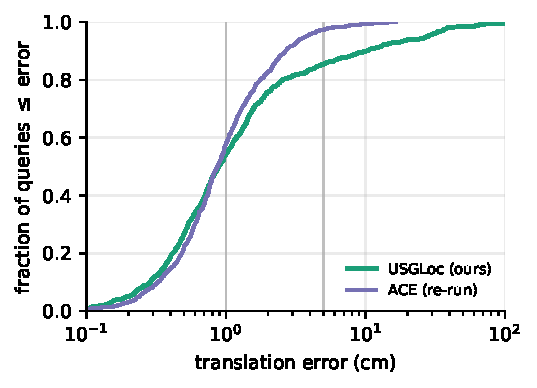
\includegraphics[width=0.9\columnwidth]{fig6_cdf.pdf}
\caption{Per-query translation-error CDF on the 700 paired test queries,
\method{} against ACE re-run with its own solver on identical frames.
\method{} has more of the most precise queries (26\% against 22\% under 0.5\,cm), ACE more under 1\,cm (58\% against 54\%) and a much shorter failure tail (3\% against 15\% beyond 5\,cm). Our residual error is concentrated in a tail of failures rather than spread over all queries, which is the regime in which a reported covariance matters; Sec.~\ref{sec:benefit} shows that the covariance identifies that tail.}
\label{fig:cdf}
\end{figure}

The convergence-versus-iteration comparison with and without the pixel
weight is not plotted separately: its end-to-end effect is the
$\gamma{=}0$ row of Table~\ref{tab:ablation-full}, and the snapped
hypotheses start within about 1\,cm of the optimum, so the refinement
trajectory is short and its shape carries little information.

\section*{Reproducibility}
All numbers in this report regenerate from the released code:
\texttt{train\_map.py} (Sec.~\ref{sec:impl}--\ref{sec:mapstats}),
\texttt{train\_encoders.py} (Sec.~\ref{sec:retrieval}), and
\texttt{run\_7scenes.py} (Sec.~\ref{sec:results}); the correction-floor, basin, map-selection, prior-refinement and baseline tables are produced by the scripts in \texttt{scripts/analysis/} (\texttt{exp\_floor.py}, \texttt{floor\_vs\_achieved.py}, \texttt{select\_map.py}, \texttt{exp\_prior2.py}, \texttt{run\_ace\_baseline.py}, \texttt{run\_marepo\_baseline.py}) and the fusion study by \texttt{eval\_fusion.py}; the per-table commands are listed in the repository. \TODO{insert repository URL at camera-ready; the
anonymized mirror during review}

\bibliographystyle{IEEEtran}
\bibliography{references}

\end{document}
